\section{Front End} 

\begin{table}[H]
    \centering
    \begin{tabular}{m{0.6\linewidth} c}
        Una volta aperta l'applicazione l'utente può effettuare il login nel caso sia già registrato, altrimenti può registrarsi come "utente" o "proprietario parcheggio". É anche possibile evitare questo passaggio effettuando l'autenticazione mediante SSO gestita da Google, Facebook o Apple. 
        &
        {\fbox{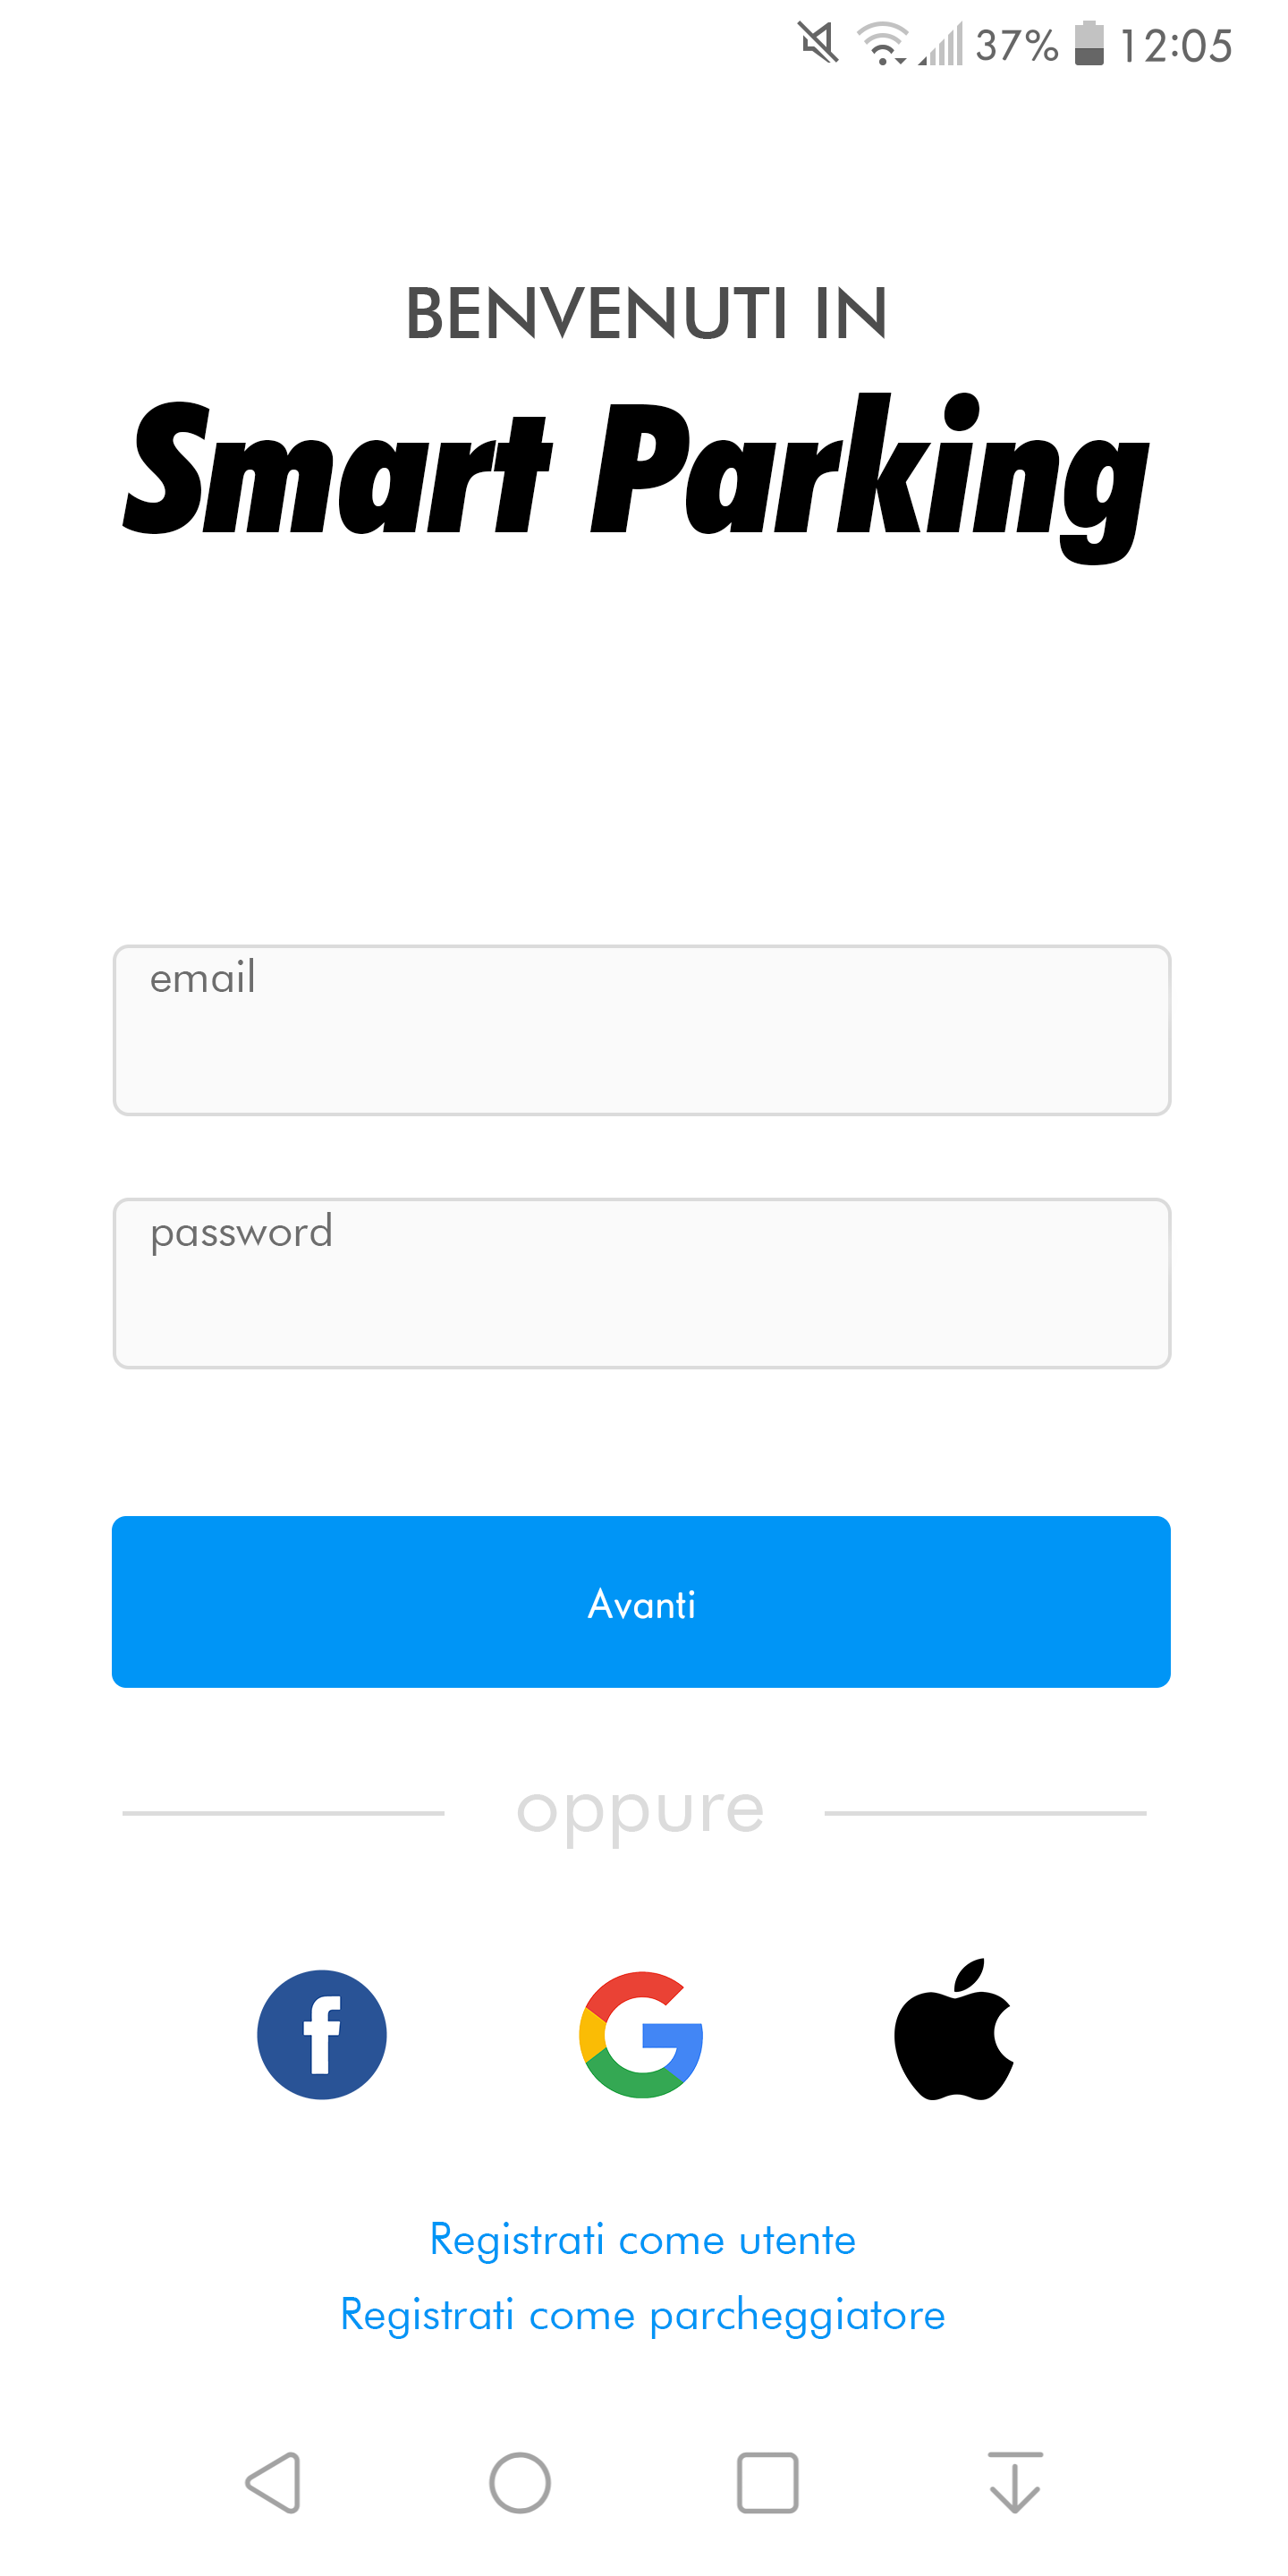
\includegraphics[scale=0.07,keepaspectratio, valign = c]{Img/primaSchermata.png}}}
        \\
    \end{tabular}
    \label{tab:login}
\end{table}
\begin{table}[H]
    \centering
    \begin{tabular}{m{0.4\linewidth} c c}
        Nel caso non si sia effettuato l'accesso con SSO, in queste due schermate vengono inseriti i dati dell'utente. All'invio dei dati, una mail di conferma viene inviata all'indirizzo email specificato contenente un link per confermare la mail, come descritto in \ref{itm:RF1} e secondo le limitazioni imposte in RNF9.1 e RNF9.2.
        &
        {\fbox{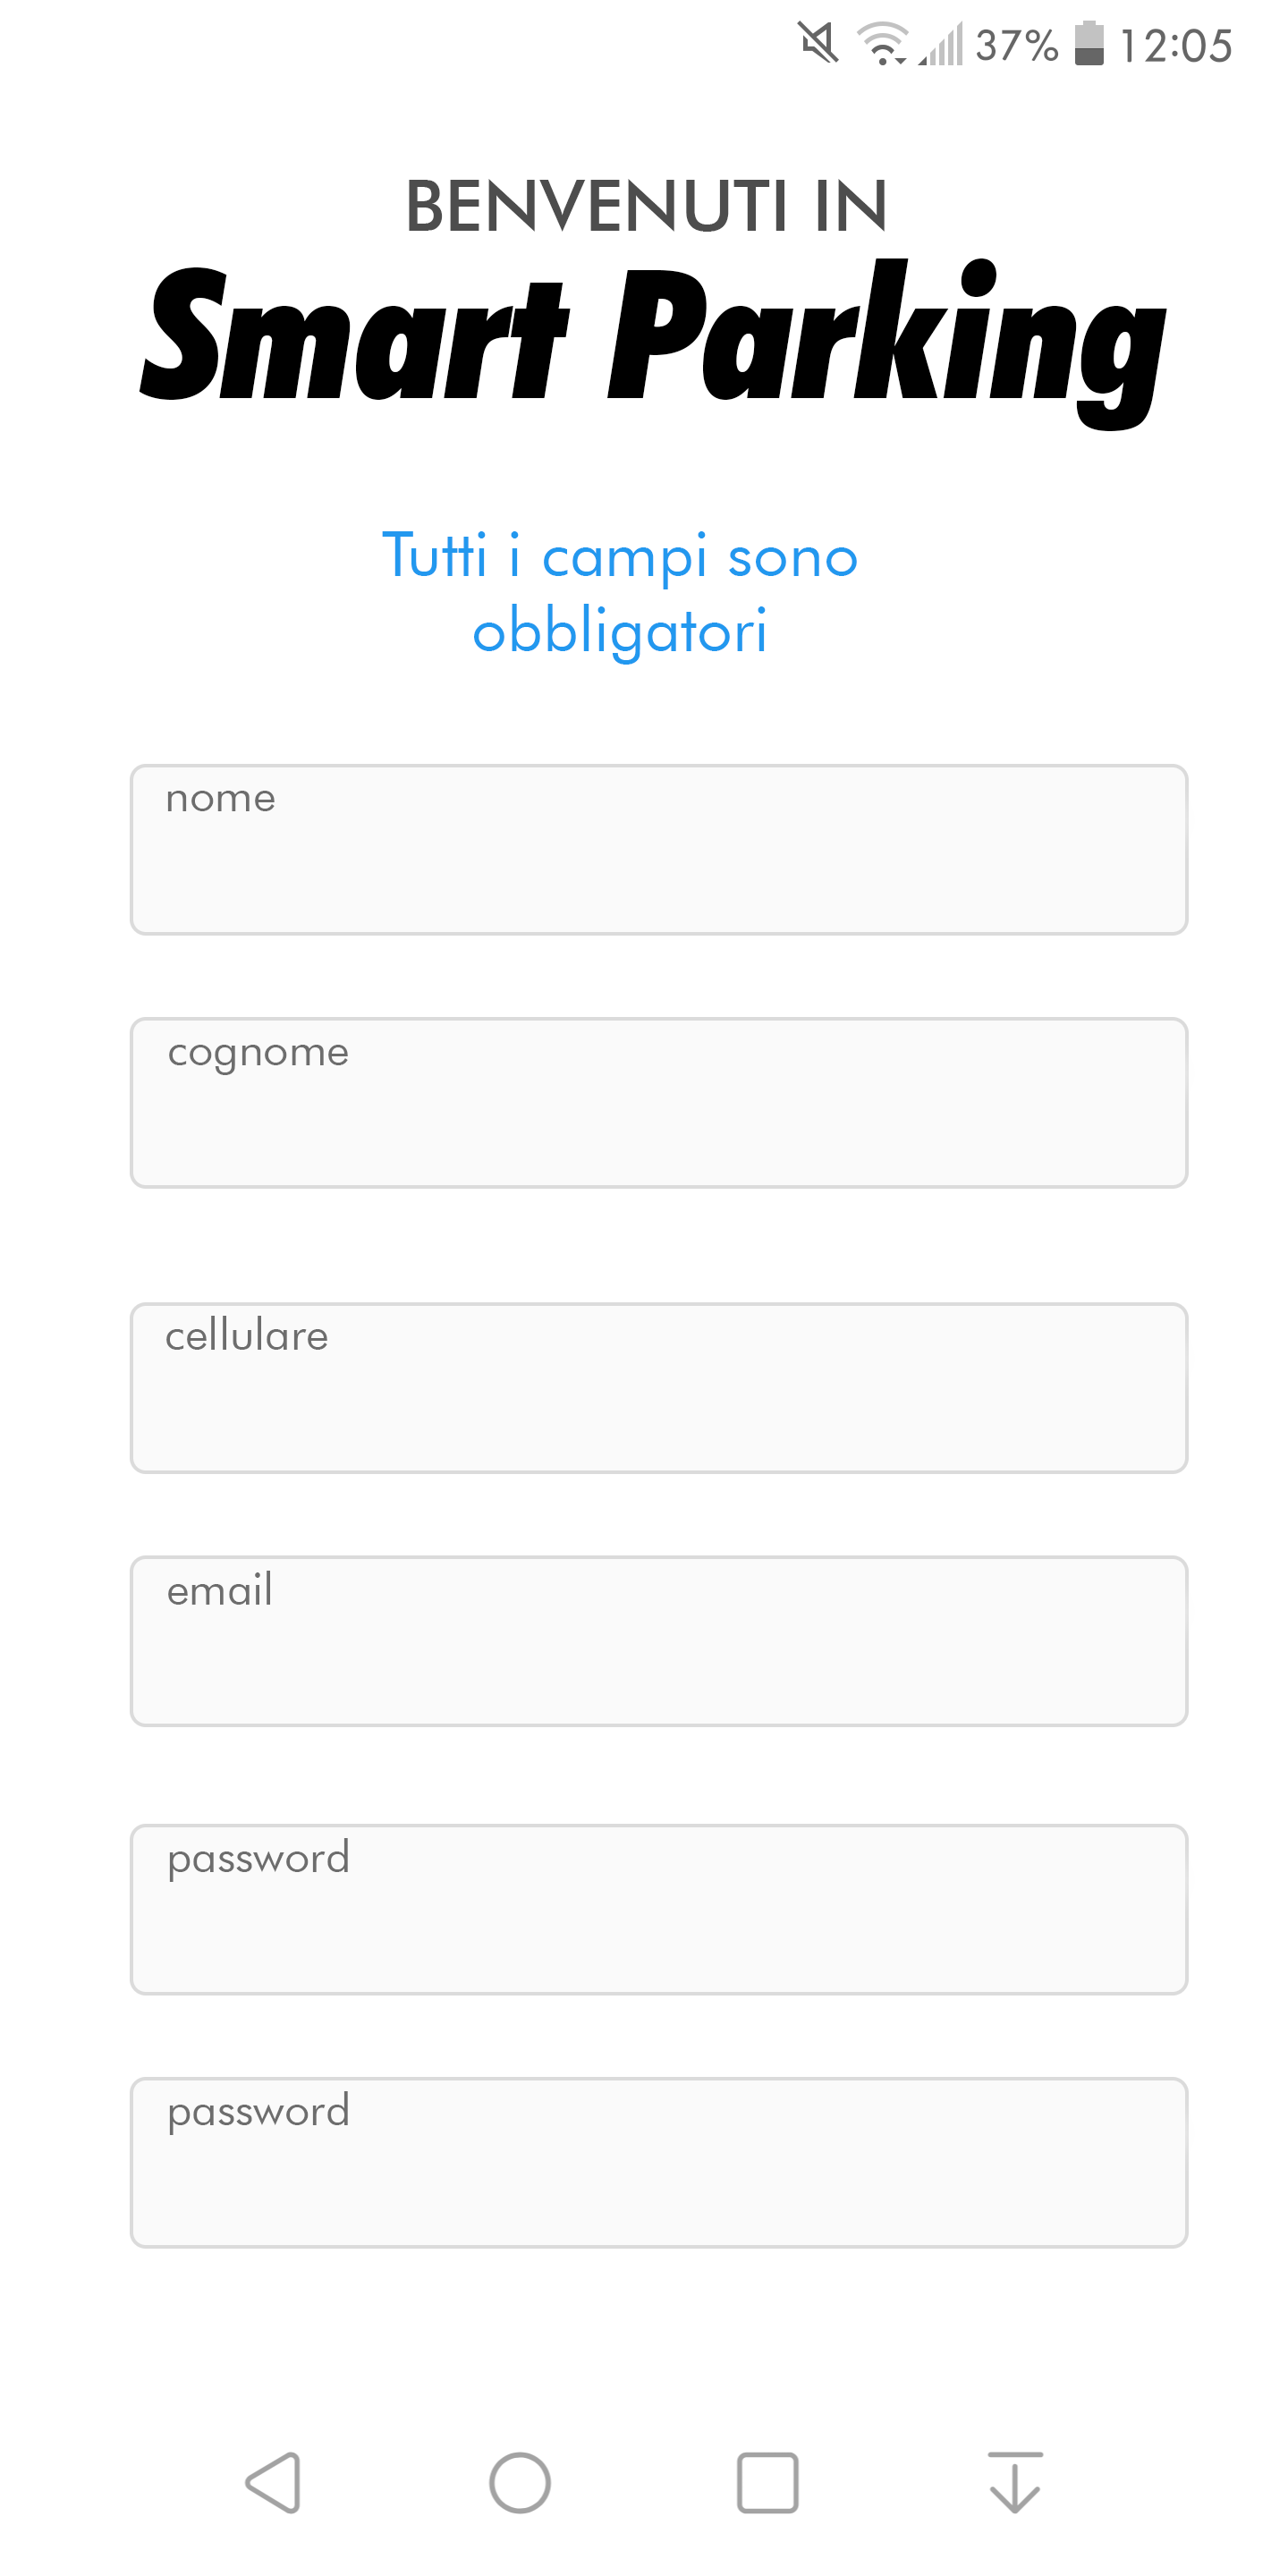
\includegraphics[scale=0.07,keepaspectratio, valign = c]{Img/registrazione1.png}}}
        &
        {\fbox{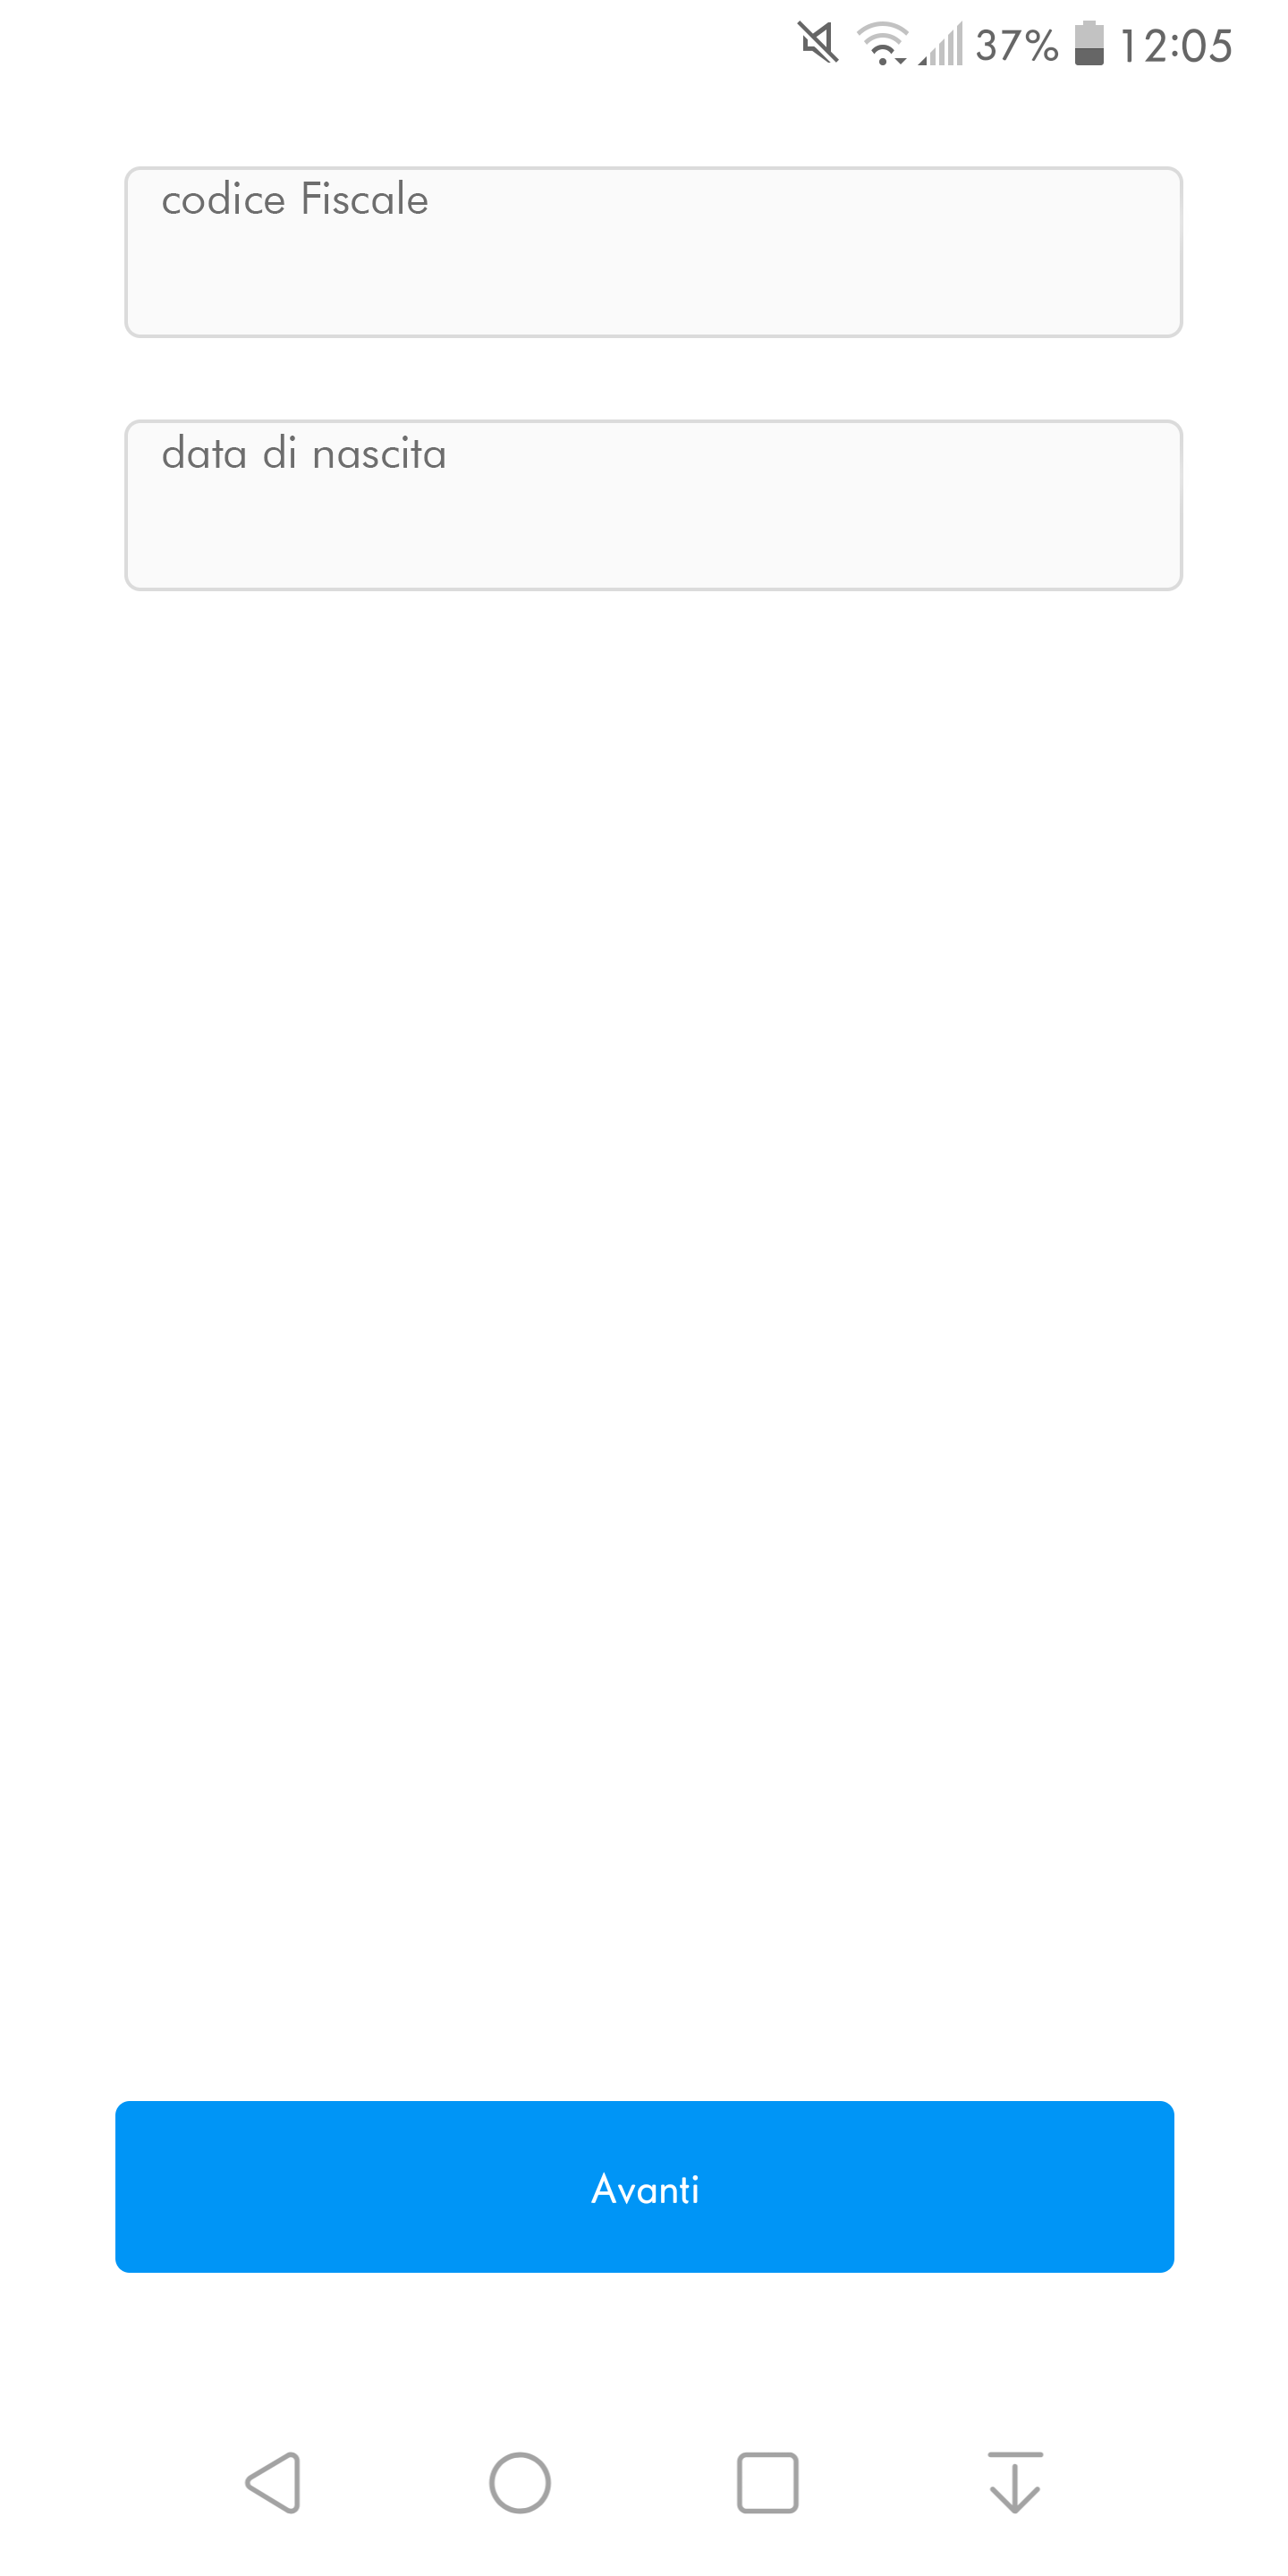
\includegraphics[scale=0.07,keepaspectratio, valign = c]{Img/registrazione2.png}}}
        \\
    \end{tabular}
    \label{tab:Registrazione}
\end{table}
\begin{table}[H]
    \centering
    \begin{tabular}{m{0.6\linewidth} c}
        Come spiegato in \ref{itm:RF4} In questa sezione l'utente autenticato inserisce le targhe delle macchine che vogliono utilizzare l'applicazione e le carte di credito utilizzate. Con il tasto "+" si può aggiungere un nuovo elemento. Entrambi i campi devono presentare almeno una componente secondo le limitazioni espresse in RNF9.3.
        &  
        {\fbox{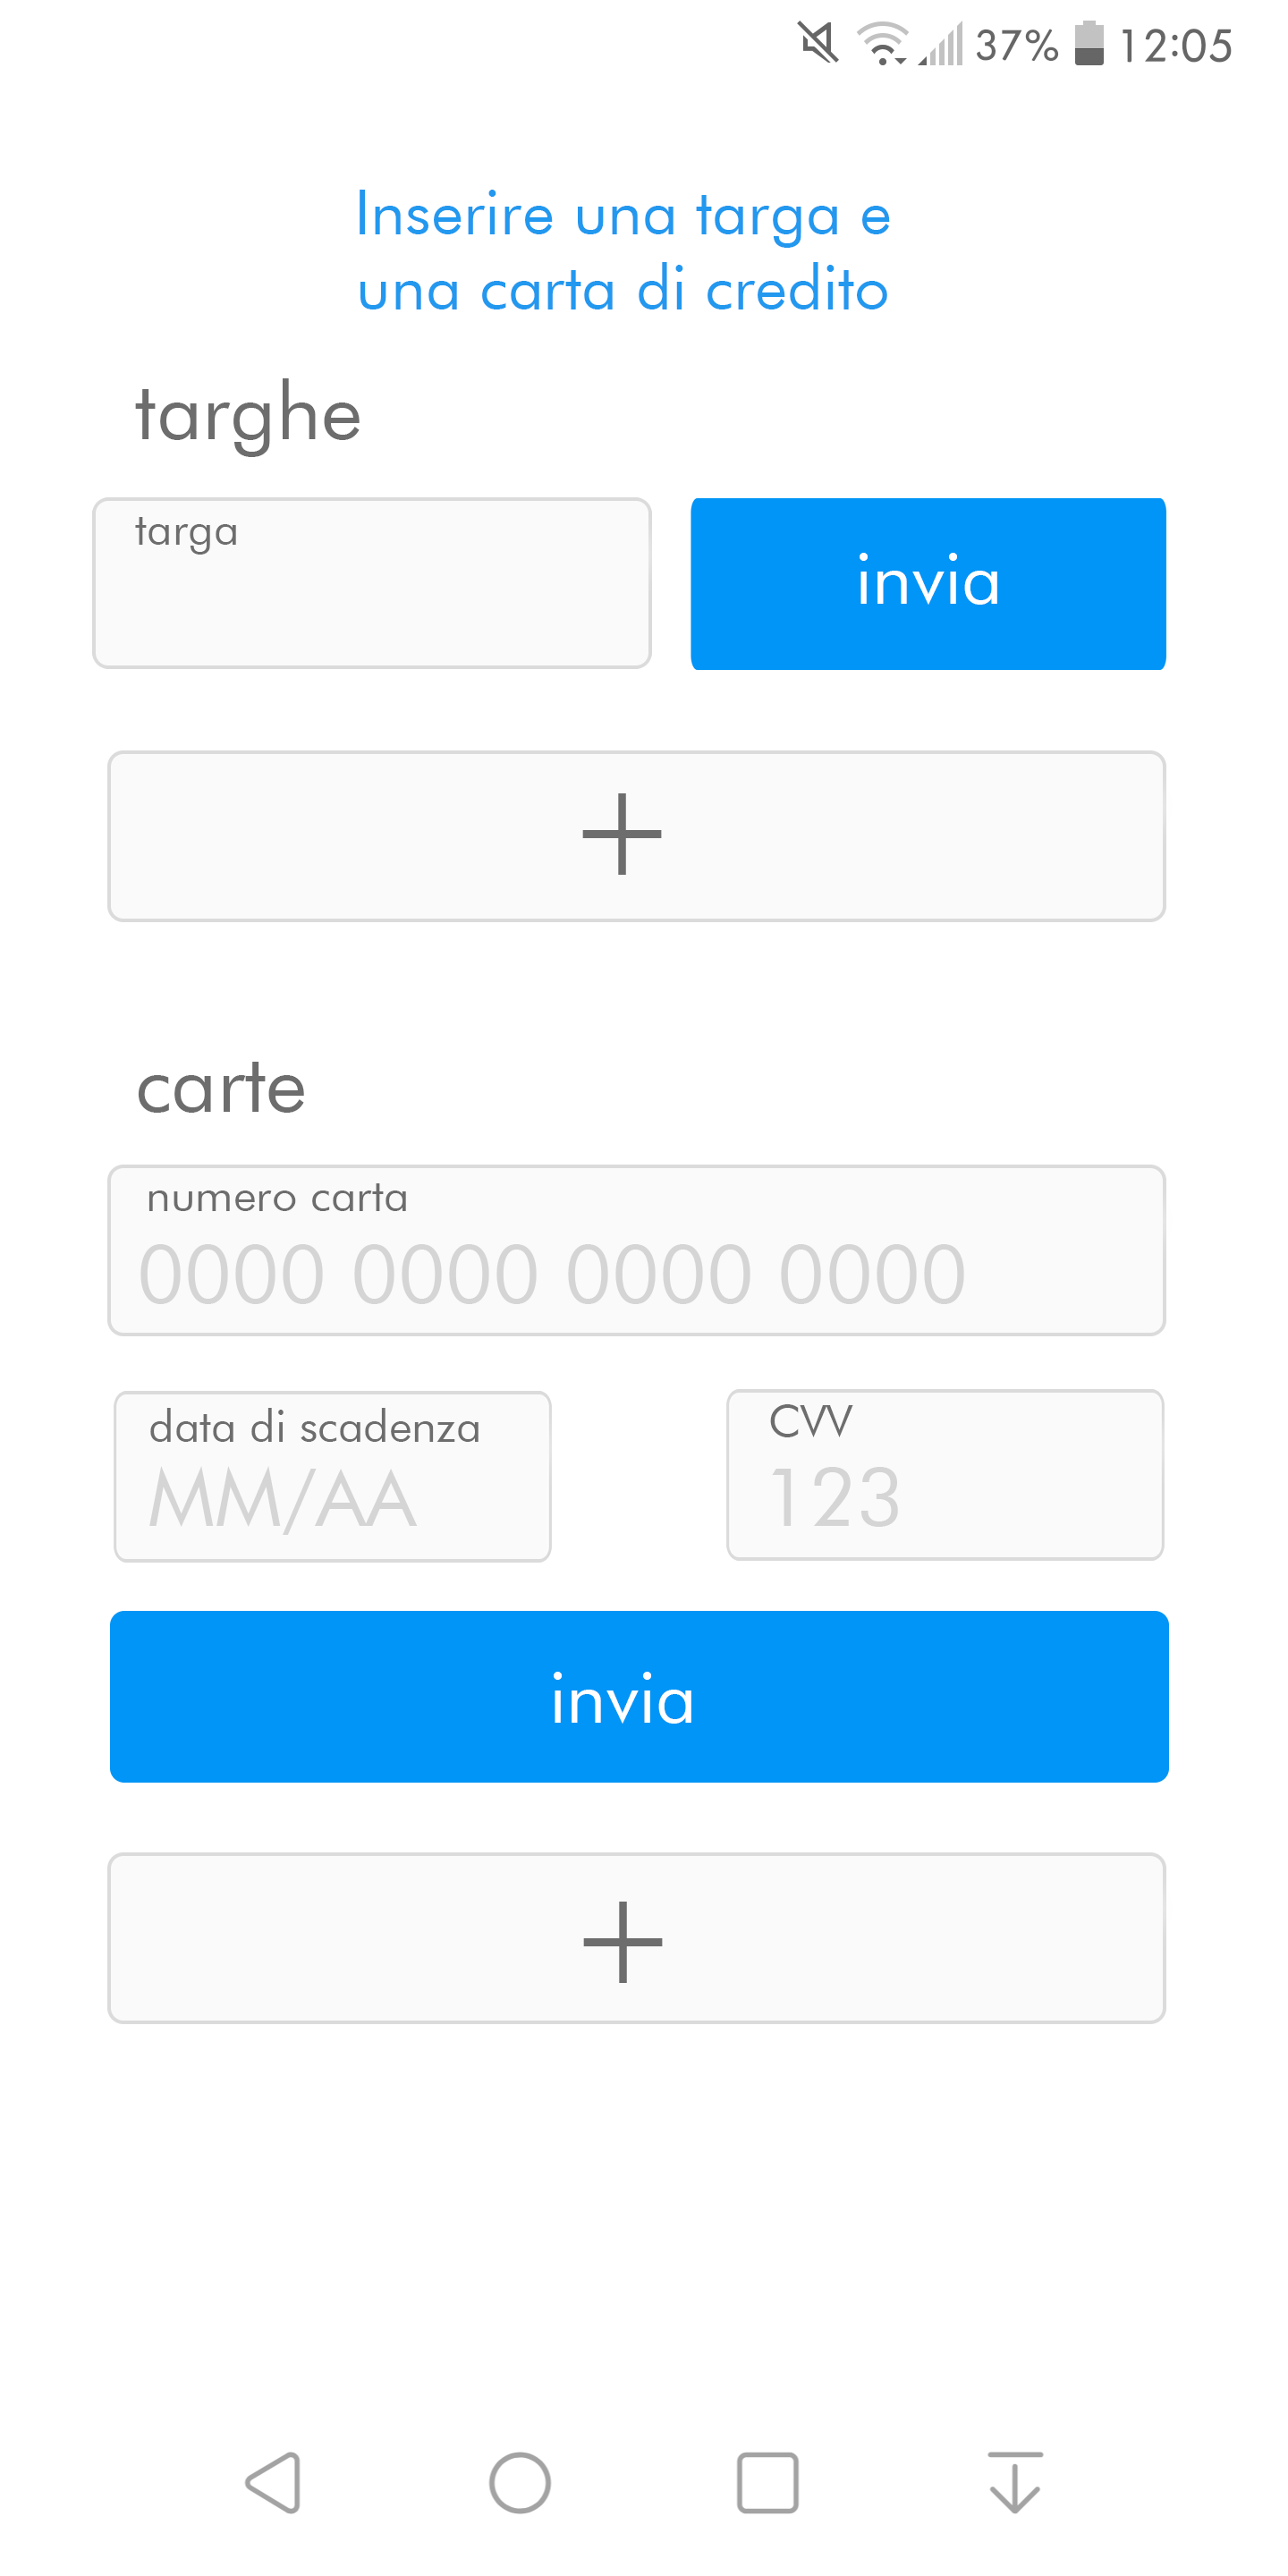
\includegraphics[scale=0.07,keepaspectratio, valign = c]{Img/cartaTargaPiu.png}}}
        \\
    \end{tabular}
    \label{tab:Targa&CC}
\end{table}
\begin{table}[H]
    \centering
    \begin{tabular}{m{0.6\linewidth} c}
        Attraverso il menù l'utente autenticato può navigare tra le schermate: "cerca parcheggio", "wallet", "prenotazioni", "possiedi un parcheggio?", "contattaci" e "logout". Inoltre, se l'utente autenticato è proprietario di uno o più parcheggi avrà a disposizione una voce nel menù ad hamburger che potrà utilizzare per gestire i suoi parcheggi.  \ref{itm:RF16}.
        &
        {\fbox{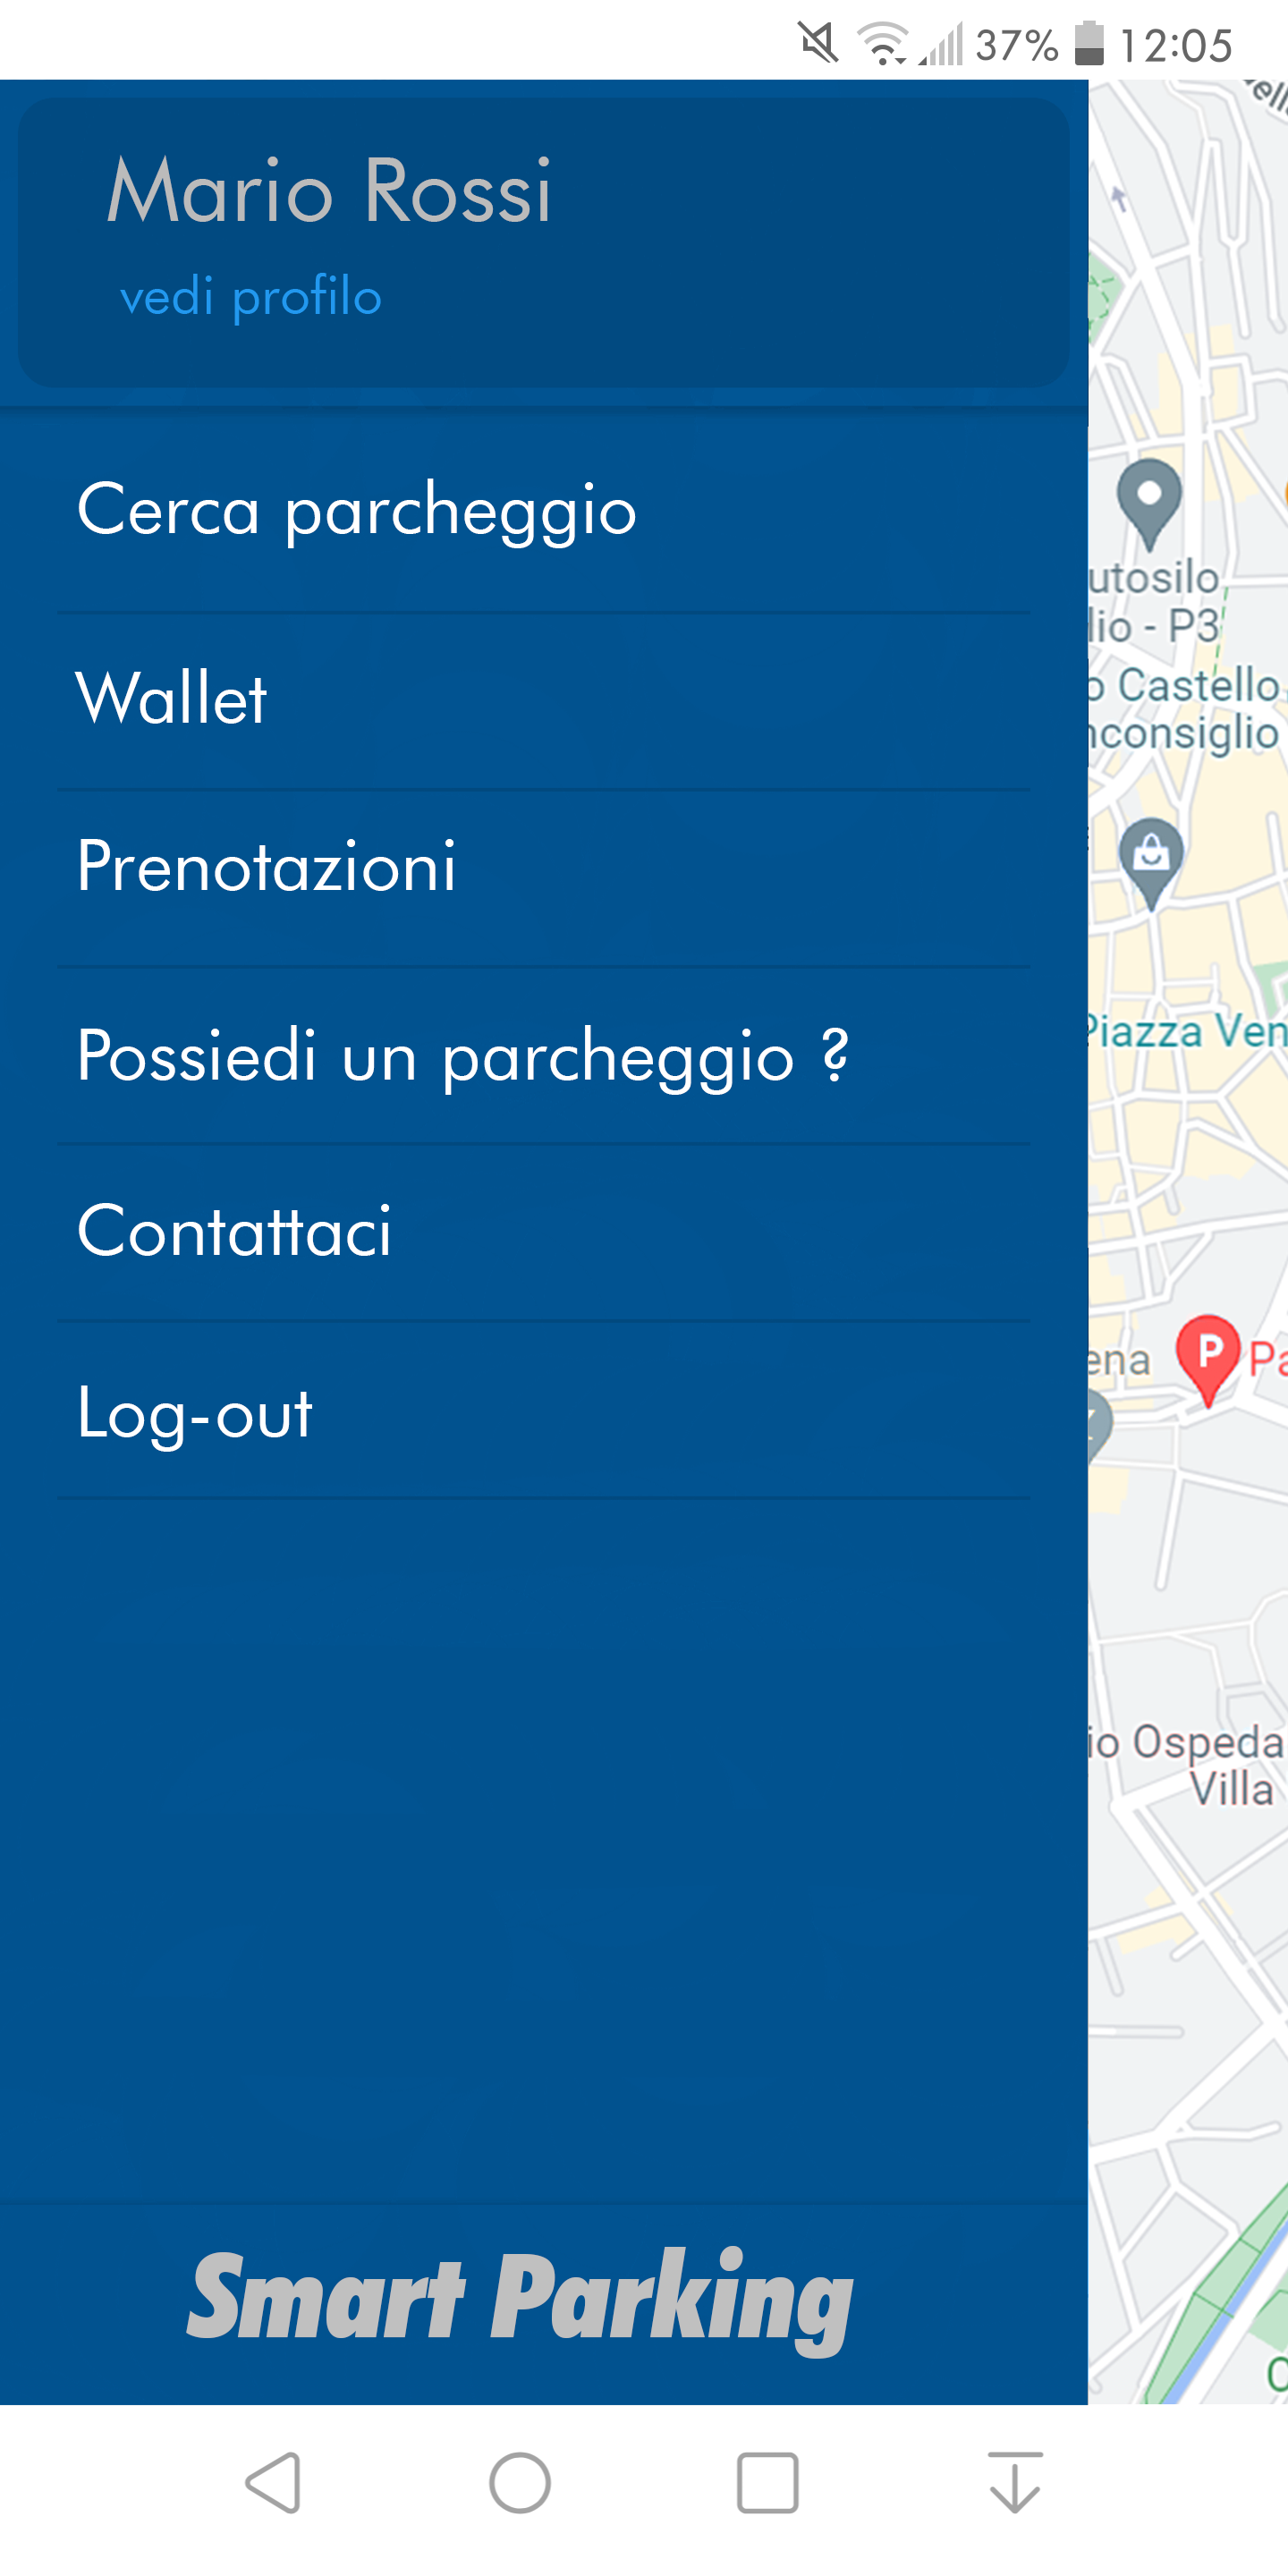
\includegraphics[scale=0.07,keepaspectratio, valign = c]{Img/menuHamburger.png}}}
        \\
    \end{tabular}
    \label{tab:Hamburger}
\end{table}
\begin{table}[H]
    \centering
    \begin{tabular}{m{0.6\linewidth} c}
        Una volta effettuato il login l'utente può interagire con google maps integrato nell'applicazione, che mostra la disponibilità dei parcheggi attraverso dei colori (verde, giallo e rosso). Selezionando la barra di ricerca l'utente può cercare un parcheggio secondo le indicazioni riportate nella figura di ricerca.
        & 
        {\fbox{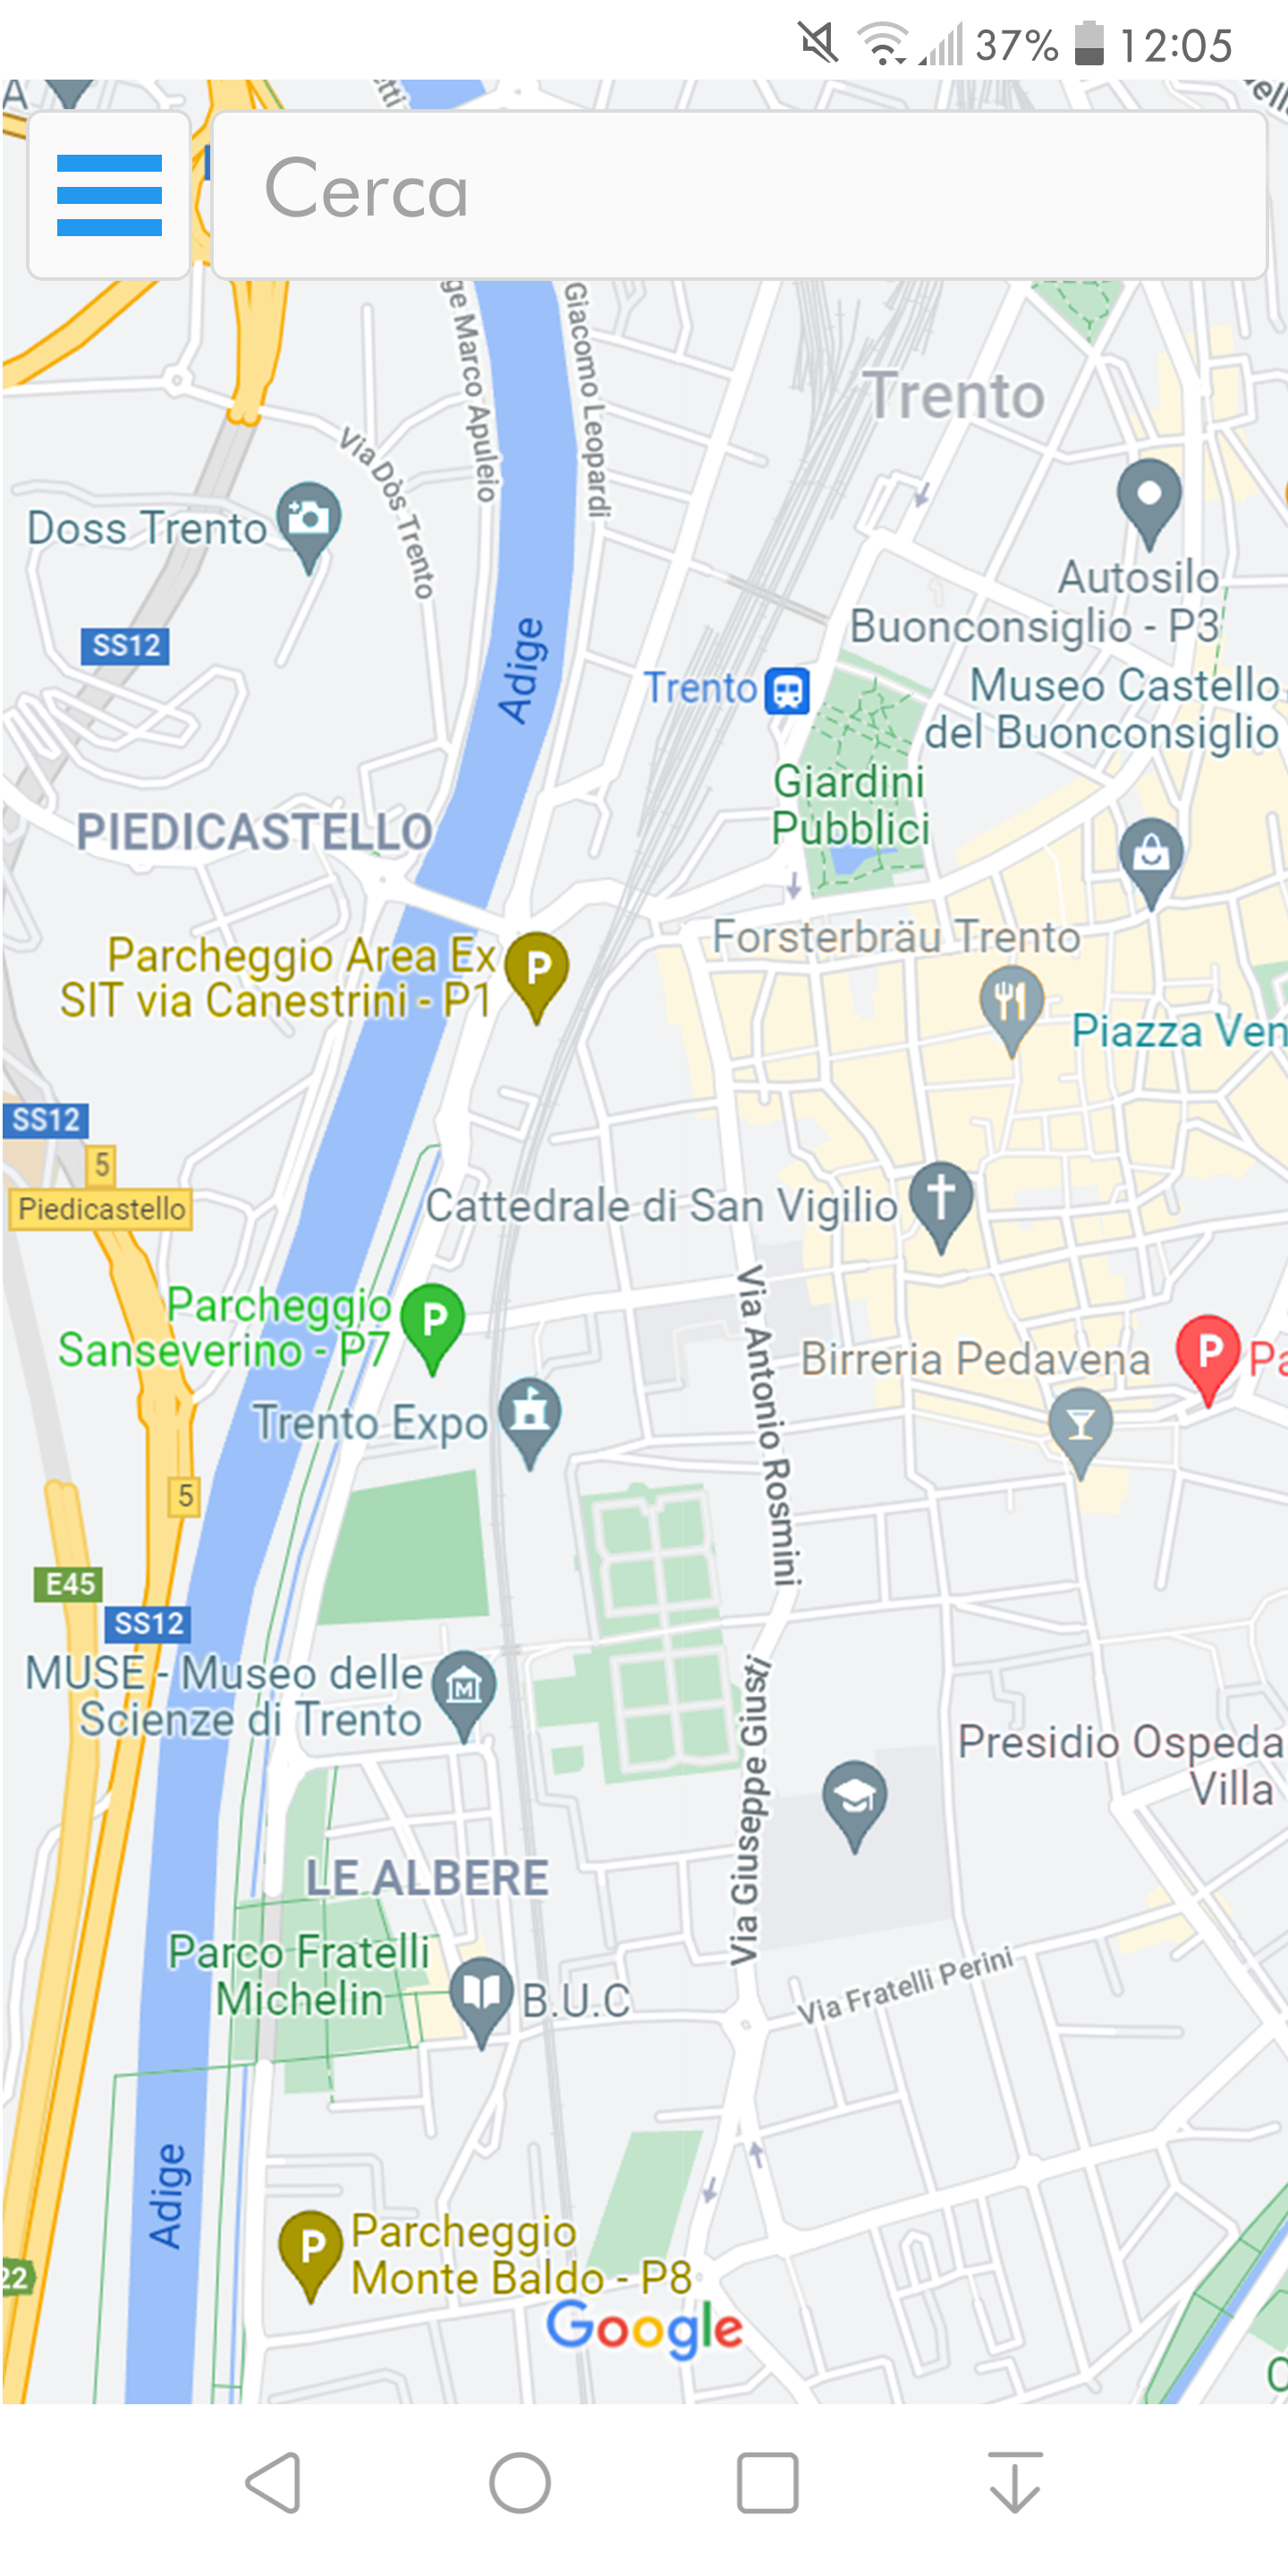
\includegraphics[scale=0.07,keepaspectratio, valign = c]{Img/home.png}}}
        \\ 
    \end{tabular}
    \label{tab:Home}
\end{table}

\begin{table}[H]
    \centering
    \begin{tabular}{m{0.6\linewidth} c}
        É possibile effettuare la ricerca applicando dei filtri in base a tariffa oraria e raggio. Il bottone "preferiti" apre la lista dei preferiti.
        &  
        {\fbox{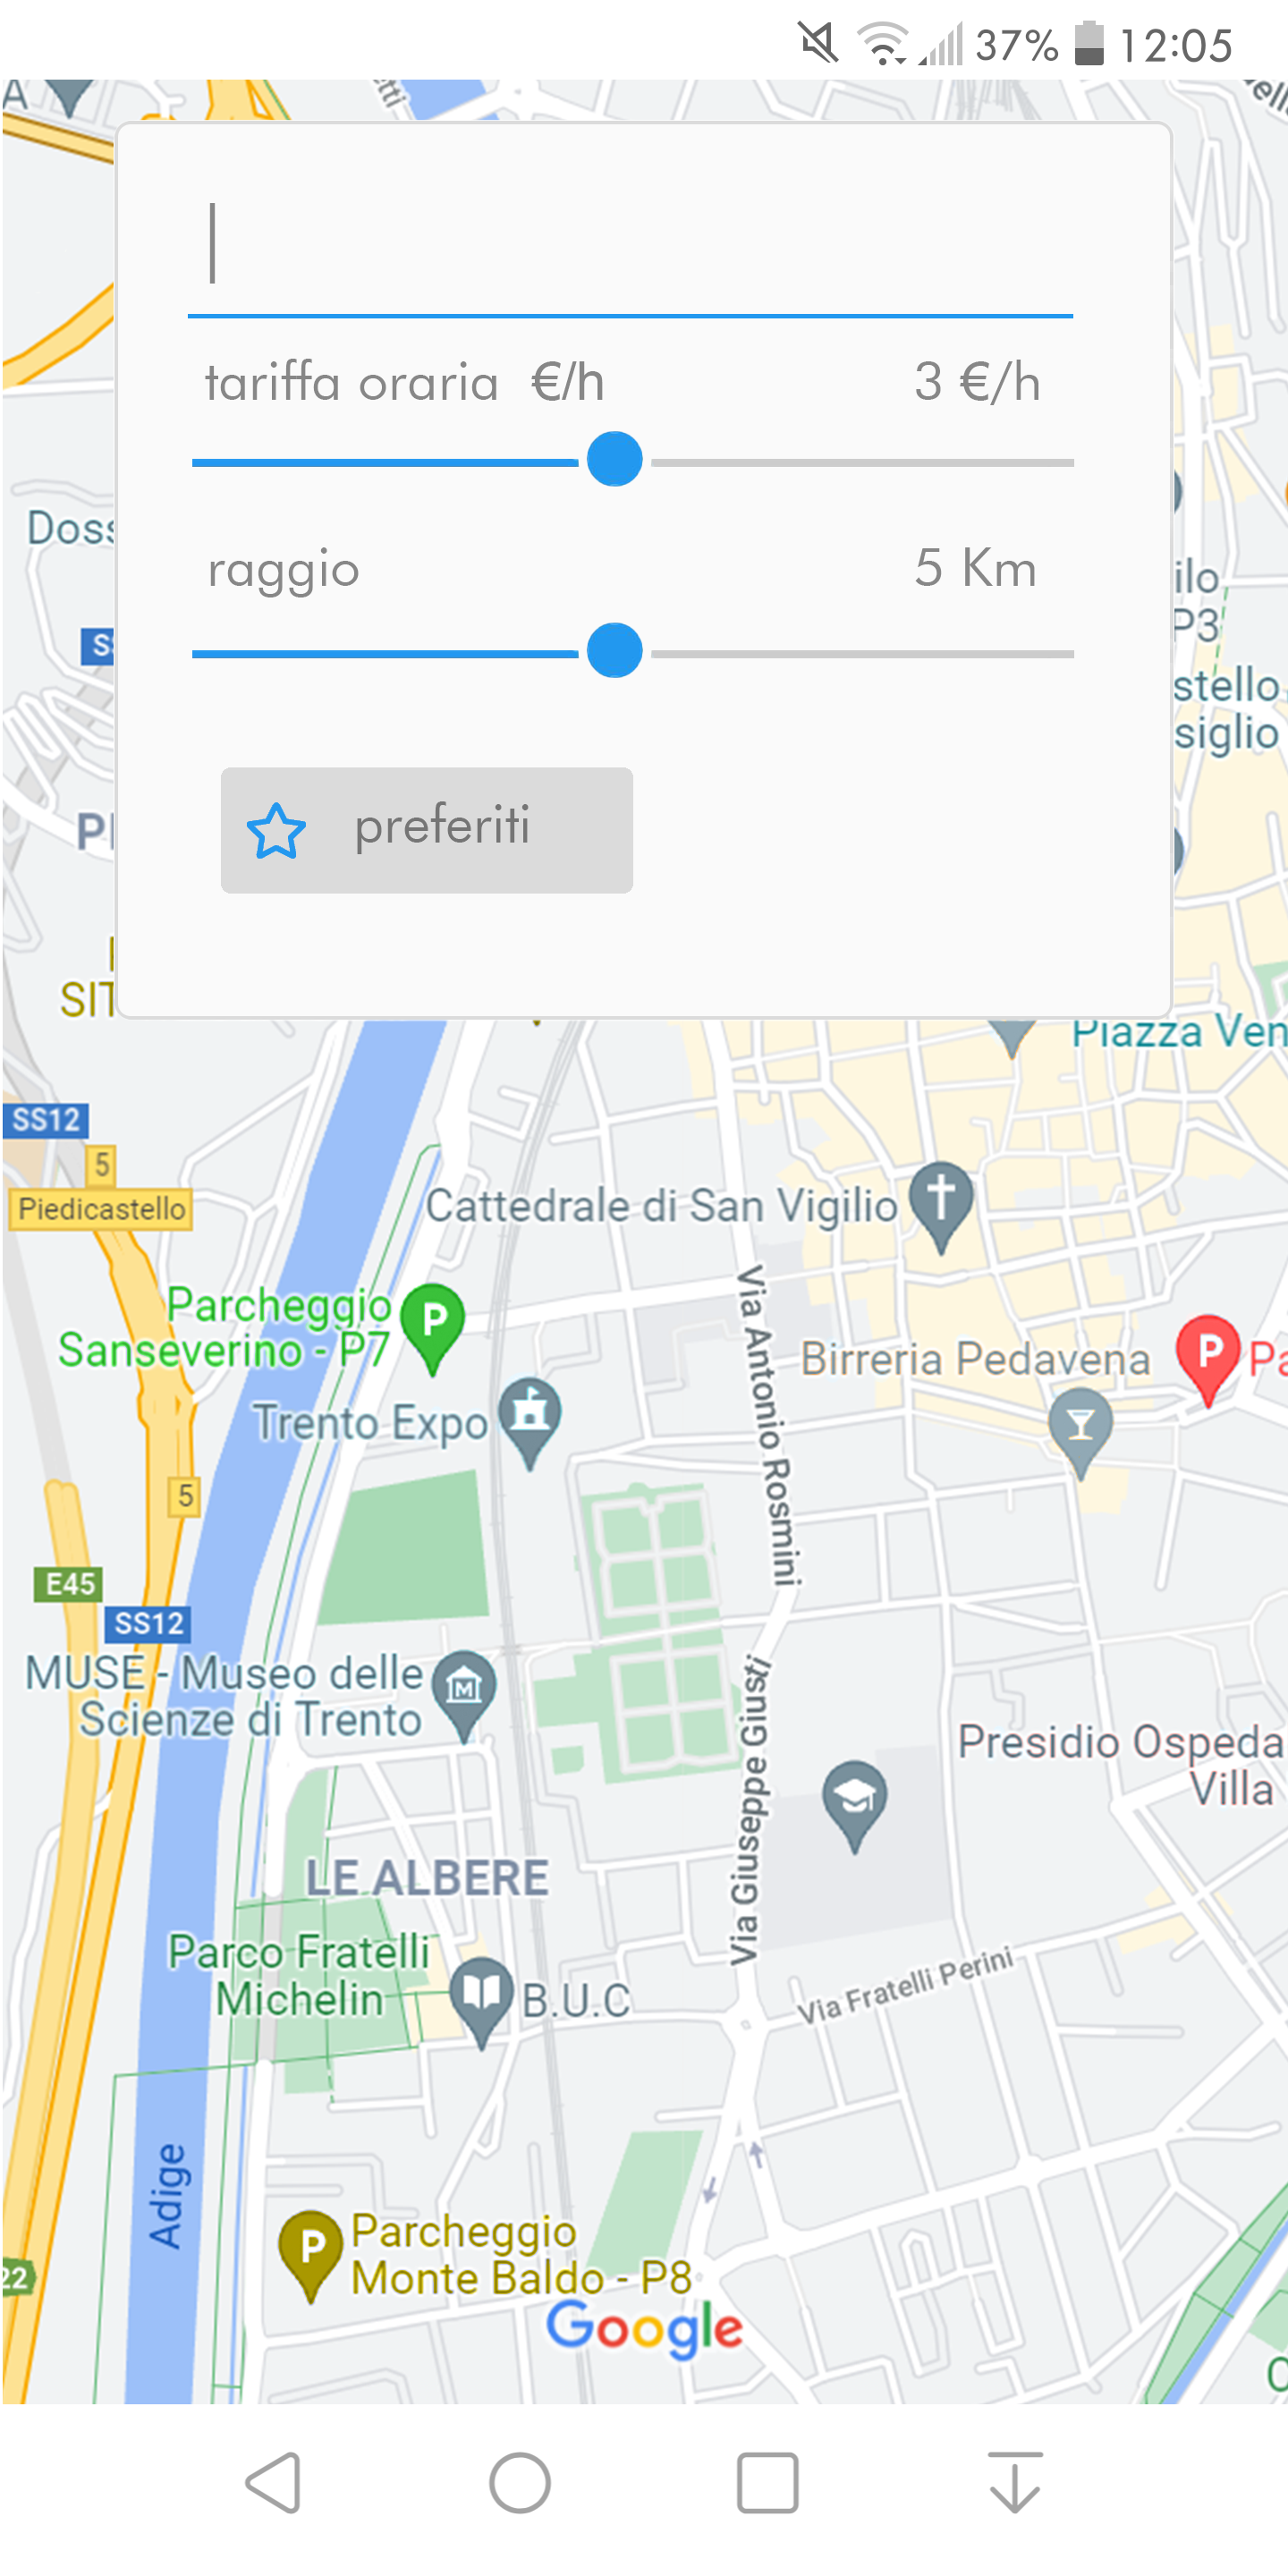
\includegraphics[scale=0.07,keepaspectratio, valign = c]{Img/ricerca.png}}} 
        \\
    \end{tabular}
    \label{tab:Ricerca}
\end{table}

\begin{table}[H]
    \centering
    \begin{tabular}{m{0.6\linewidth} c}
        Una volta effettuata la ricerca viene presentata una lista in base ai filtri applicati ed è possibile aggiungere o rimuovere i parcheggi ai preferiti. Il bottone "ordina" apre un filtro, come visto in \ref{itm:RF8}.
         &  
        {\fbox{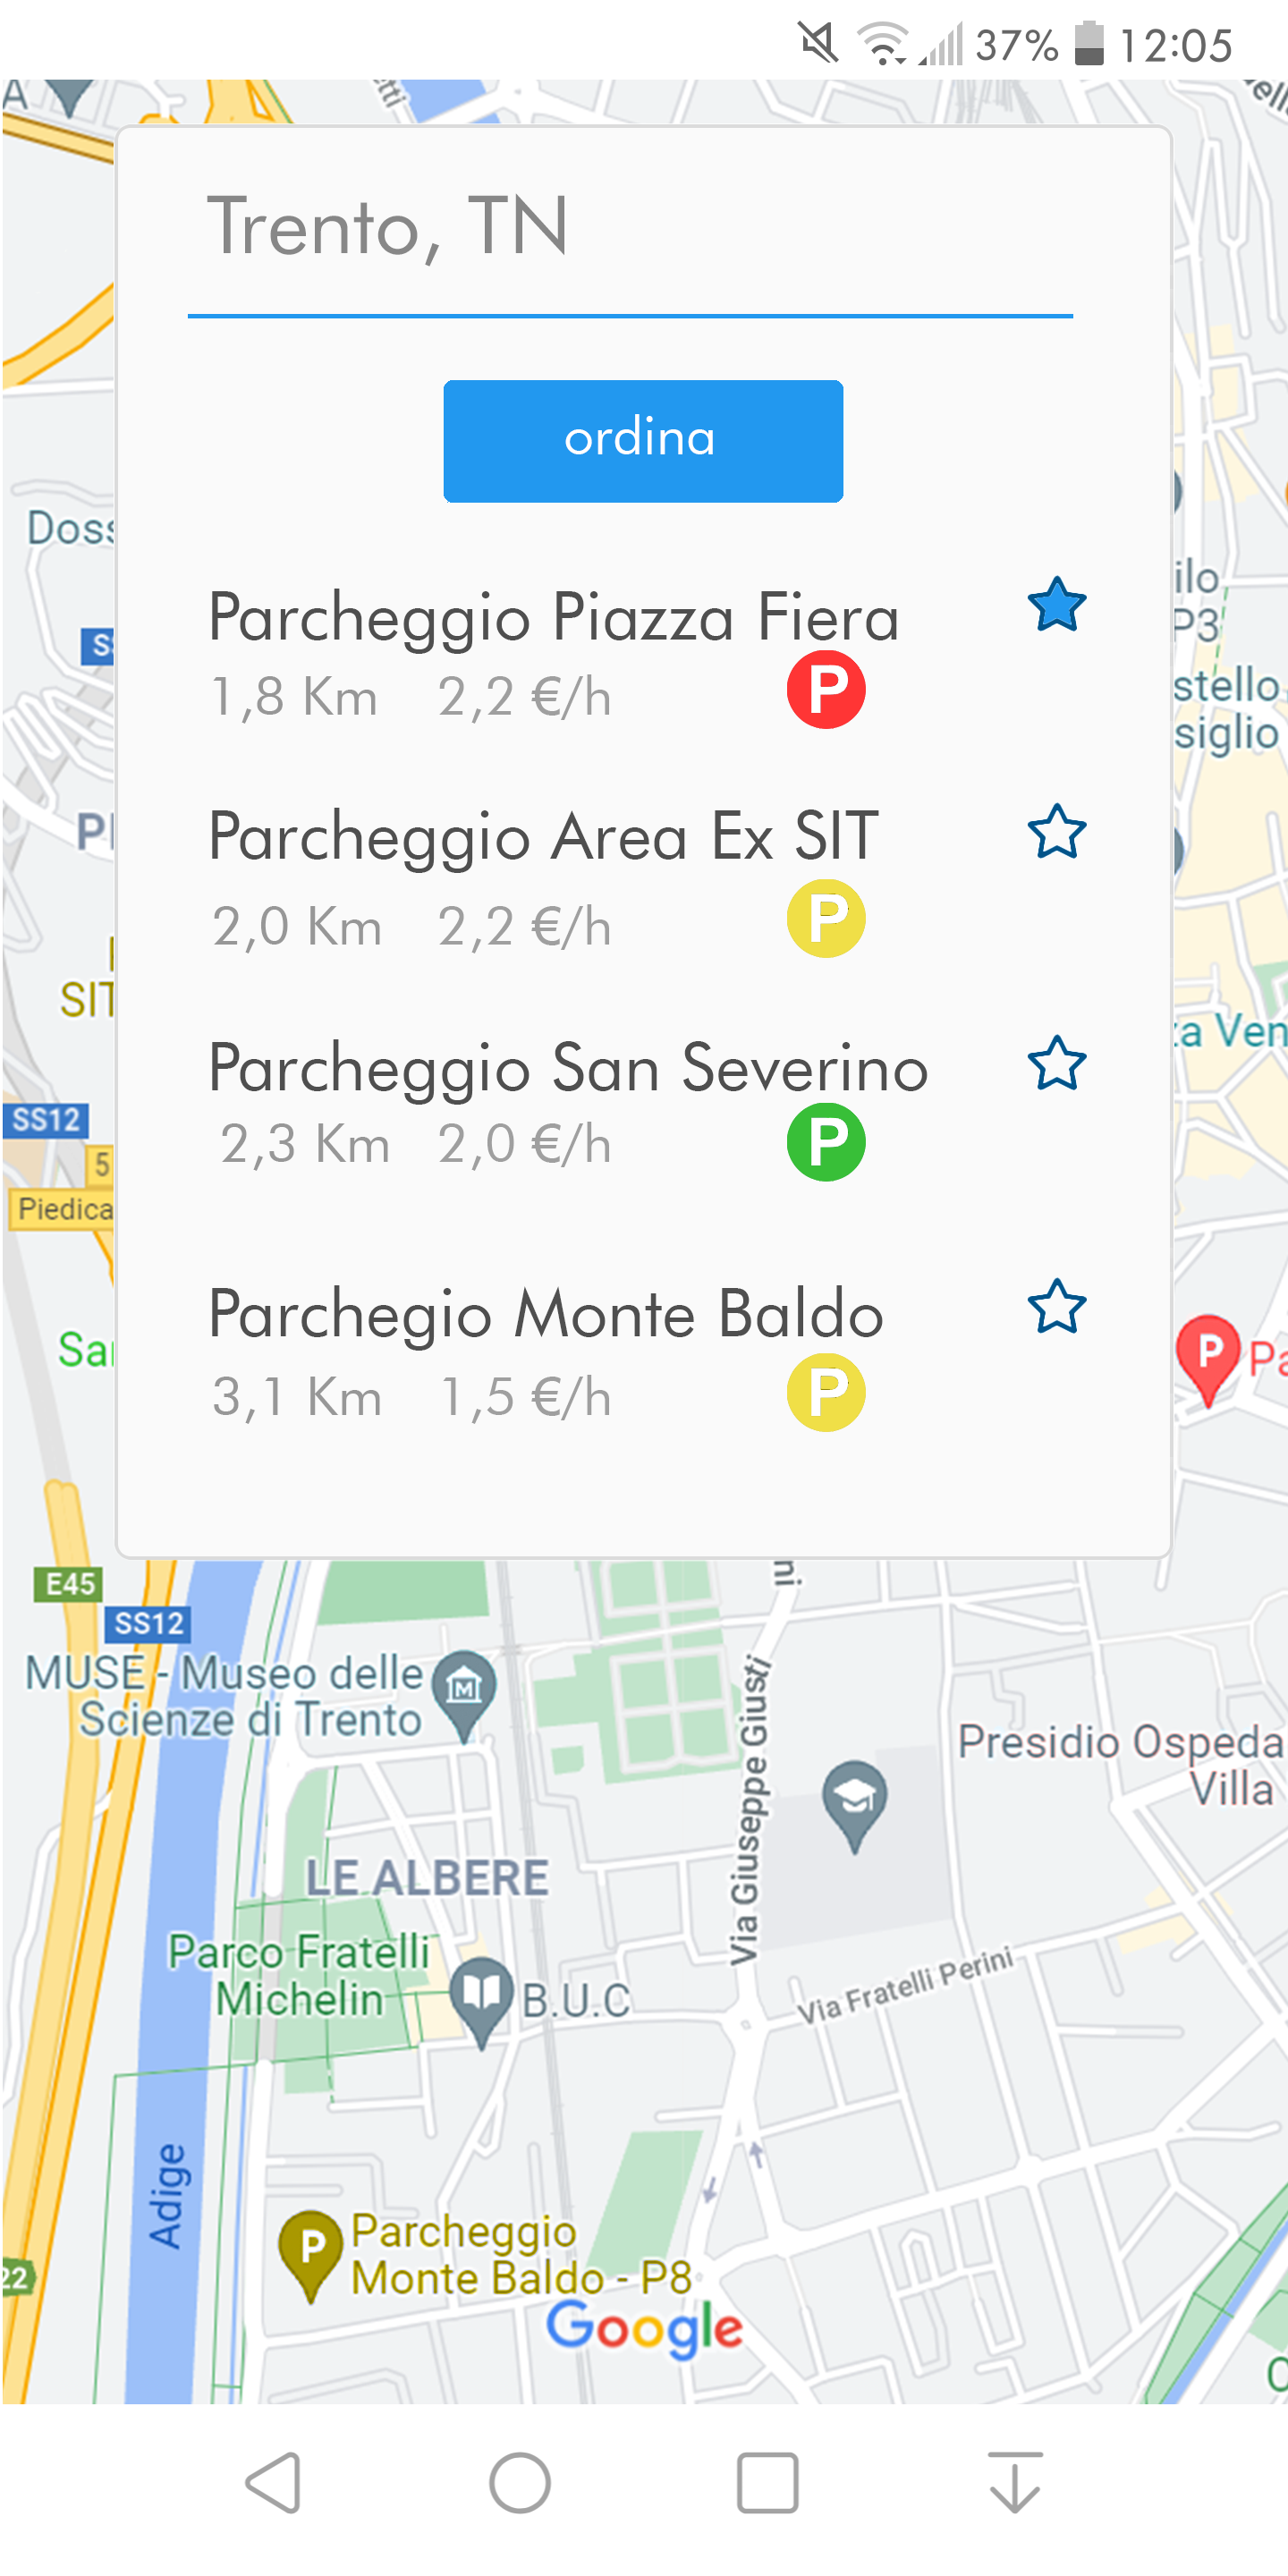
\includegraphics[scale=0.07,keepaspectratio, valign = c]{Img/ricercaFatta.png}}}
         \\
         & 
    \end{tabular}
    \label{tab:RicercaFatta}
\end{table}

\begin{table}[H]
    \centering
    \begin{tabular}{m{0.6\linewidth} c}
        Una volta selezionato un parcheggio dalla finestra precedente è possibile selezionare il tempo di sosta mediante uno slider e confermare con il tasto "prenota".
        \textcolor{red}{Se lo slider viene portato ad una durata maggiore di 24h la finestra di prenotazione si allarga includendo delle sezioni dove poter selezionare il giorno e la fascia oraria della prenotazione}. La gestione delle prenotazioni da parte del sistema è descritta in \ref{itm:RF20} e l'accettazione delle suddette è descritto secondo il \ref{itm:RF23}.
        &  
        {\fbox{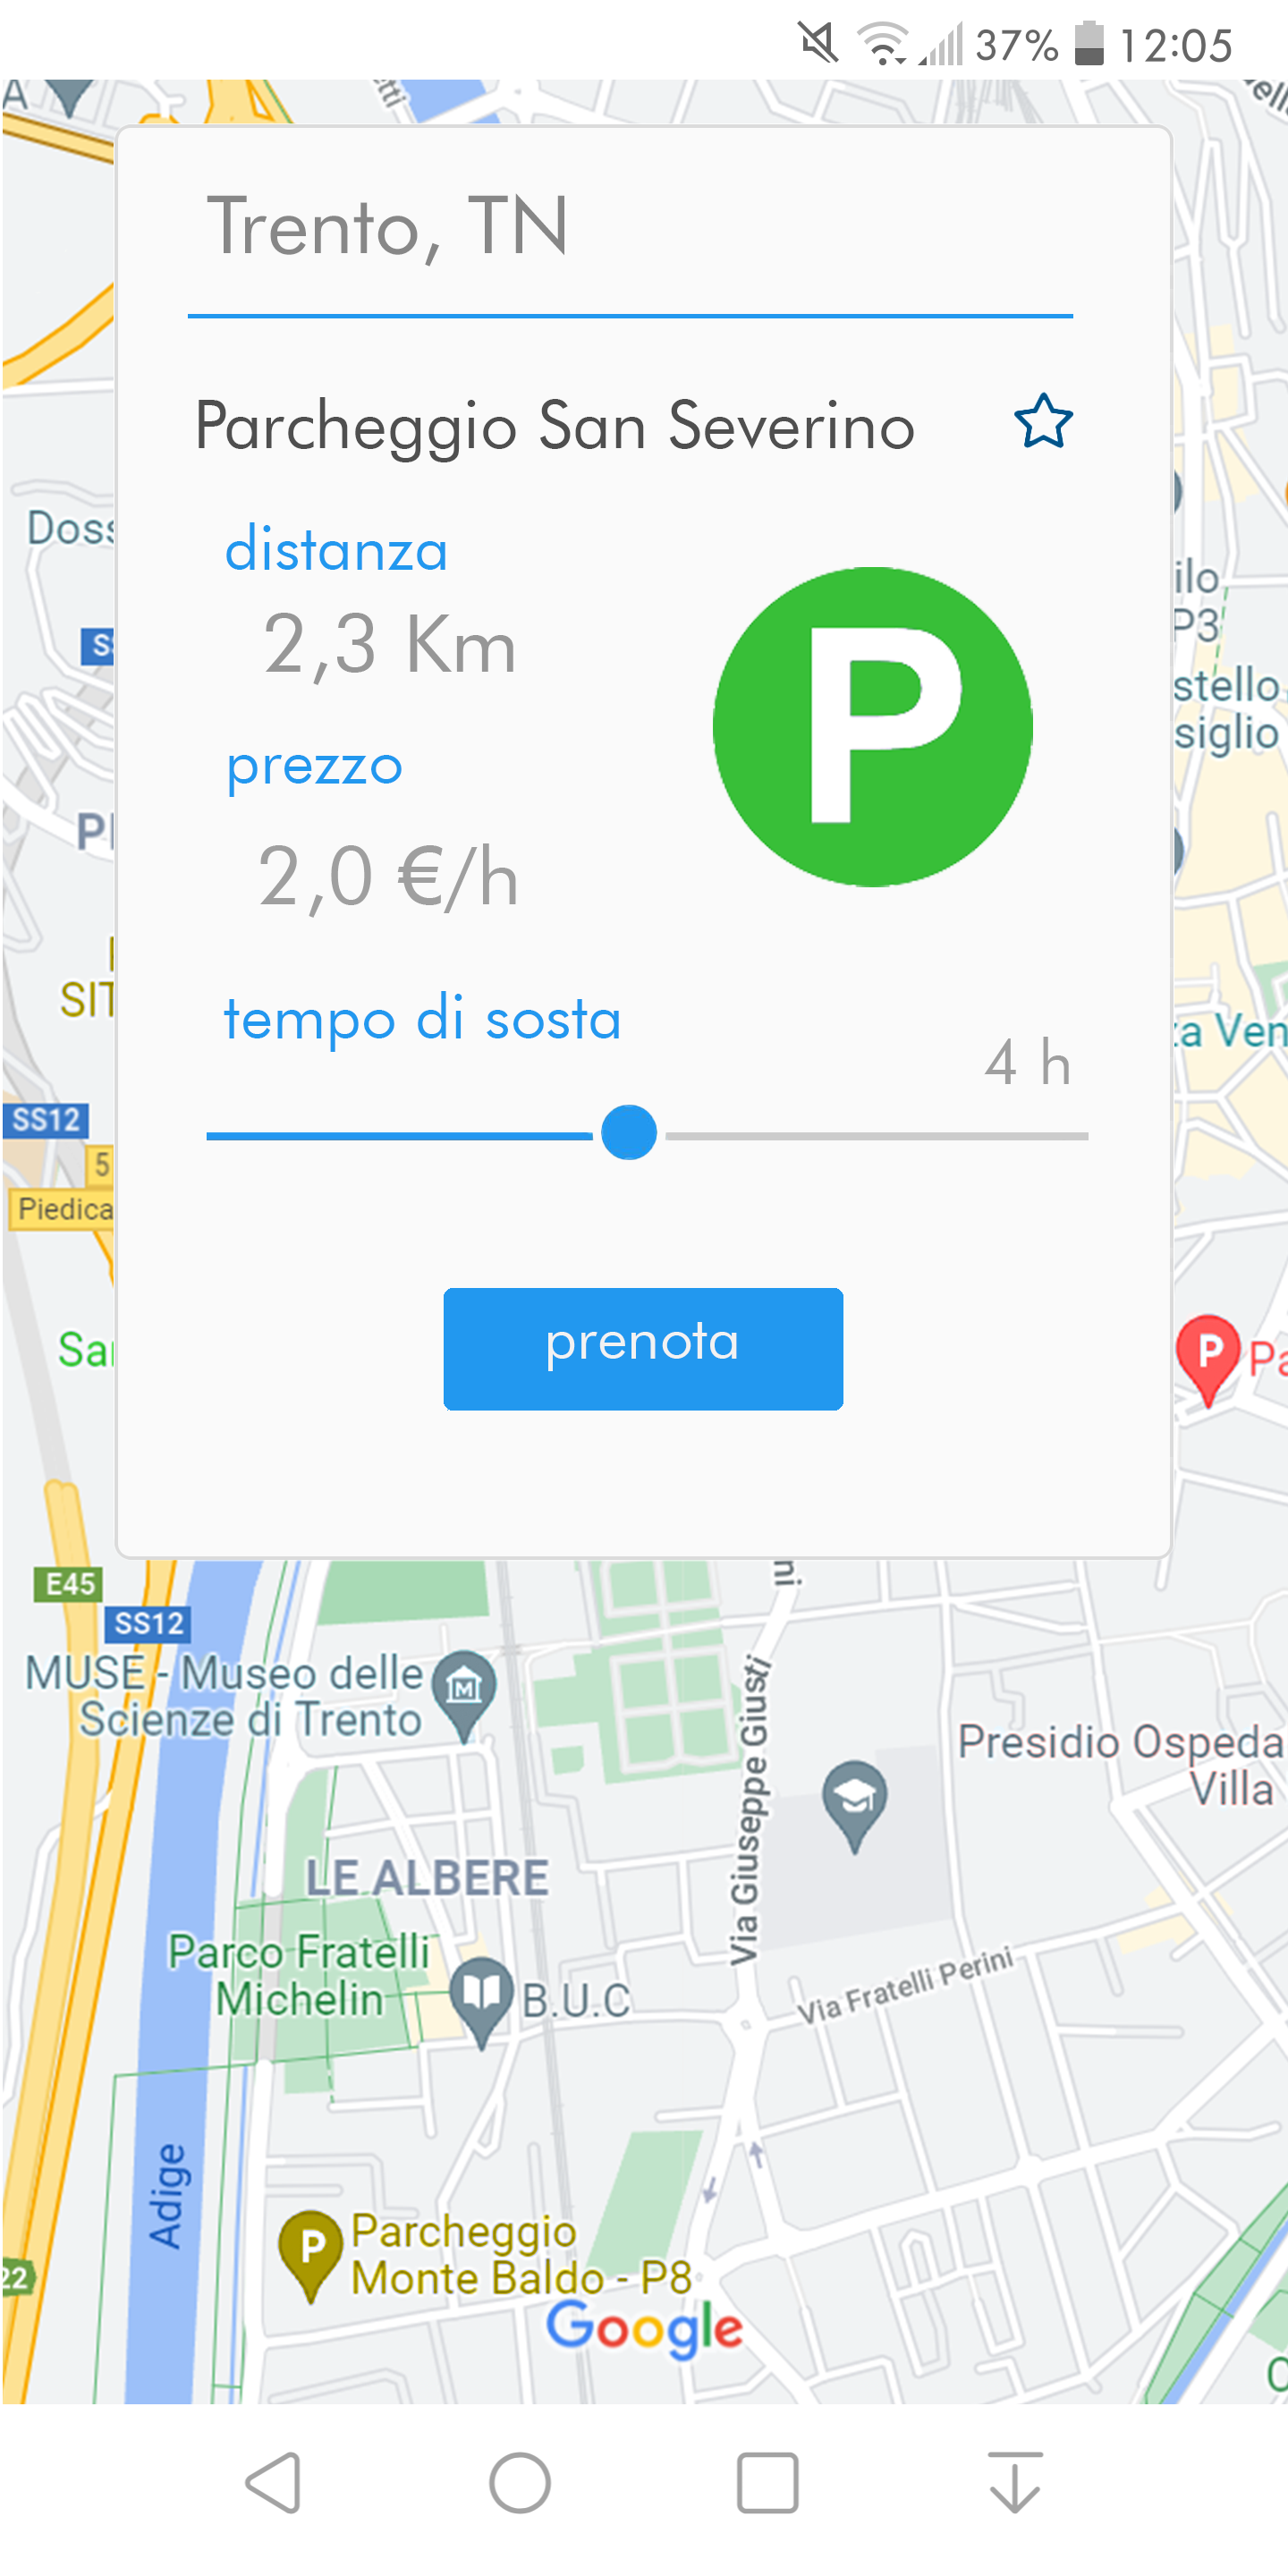
\includegraphics[scale=0.07,keepaspectratio, valign = c]{Img/prenotazione.png}}}
        \\
    \end{tabular}
    \label{tab:prenotazione}
\end{table}

\begin{table}[H]
    \centering
    \begin{tabular}{m{0.6\linewidth} c}
        In questa schermata l'utente può visionare lo stato del wallet (saldo e transazioni) ed effettuarne la ricarica tramite una carta di credito memorizzata nell'account. 
        &
        {\fbox{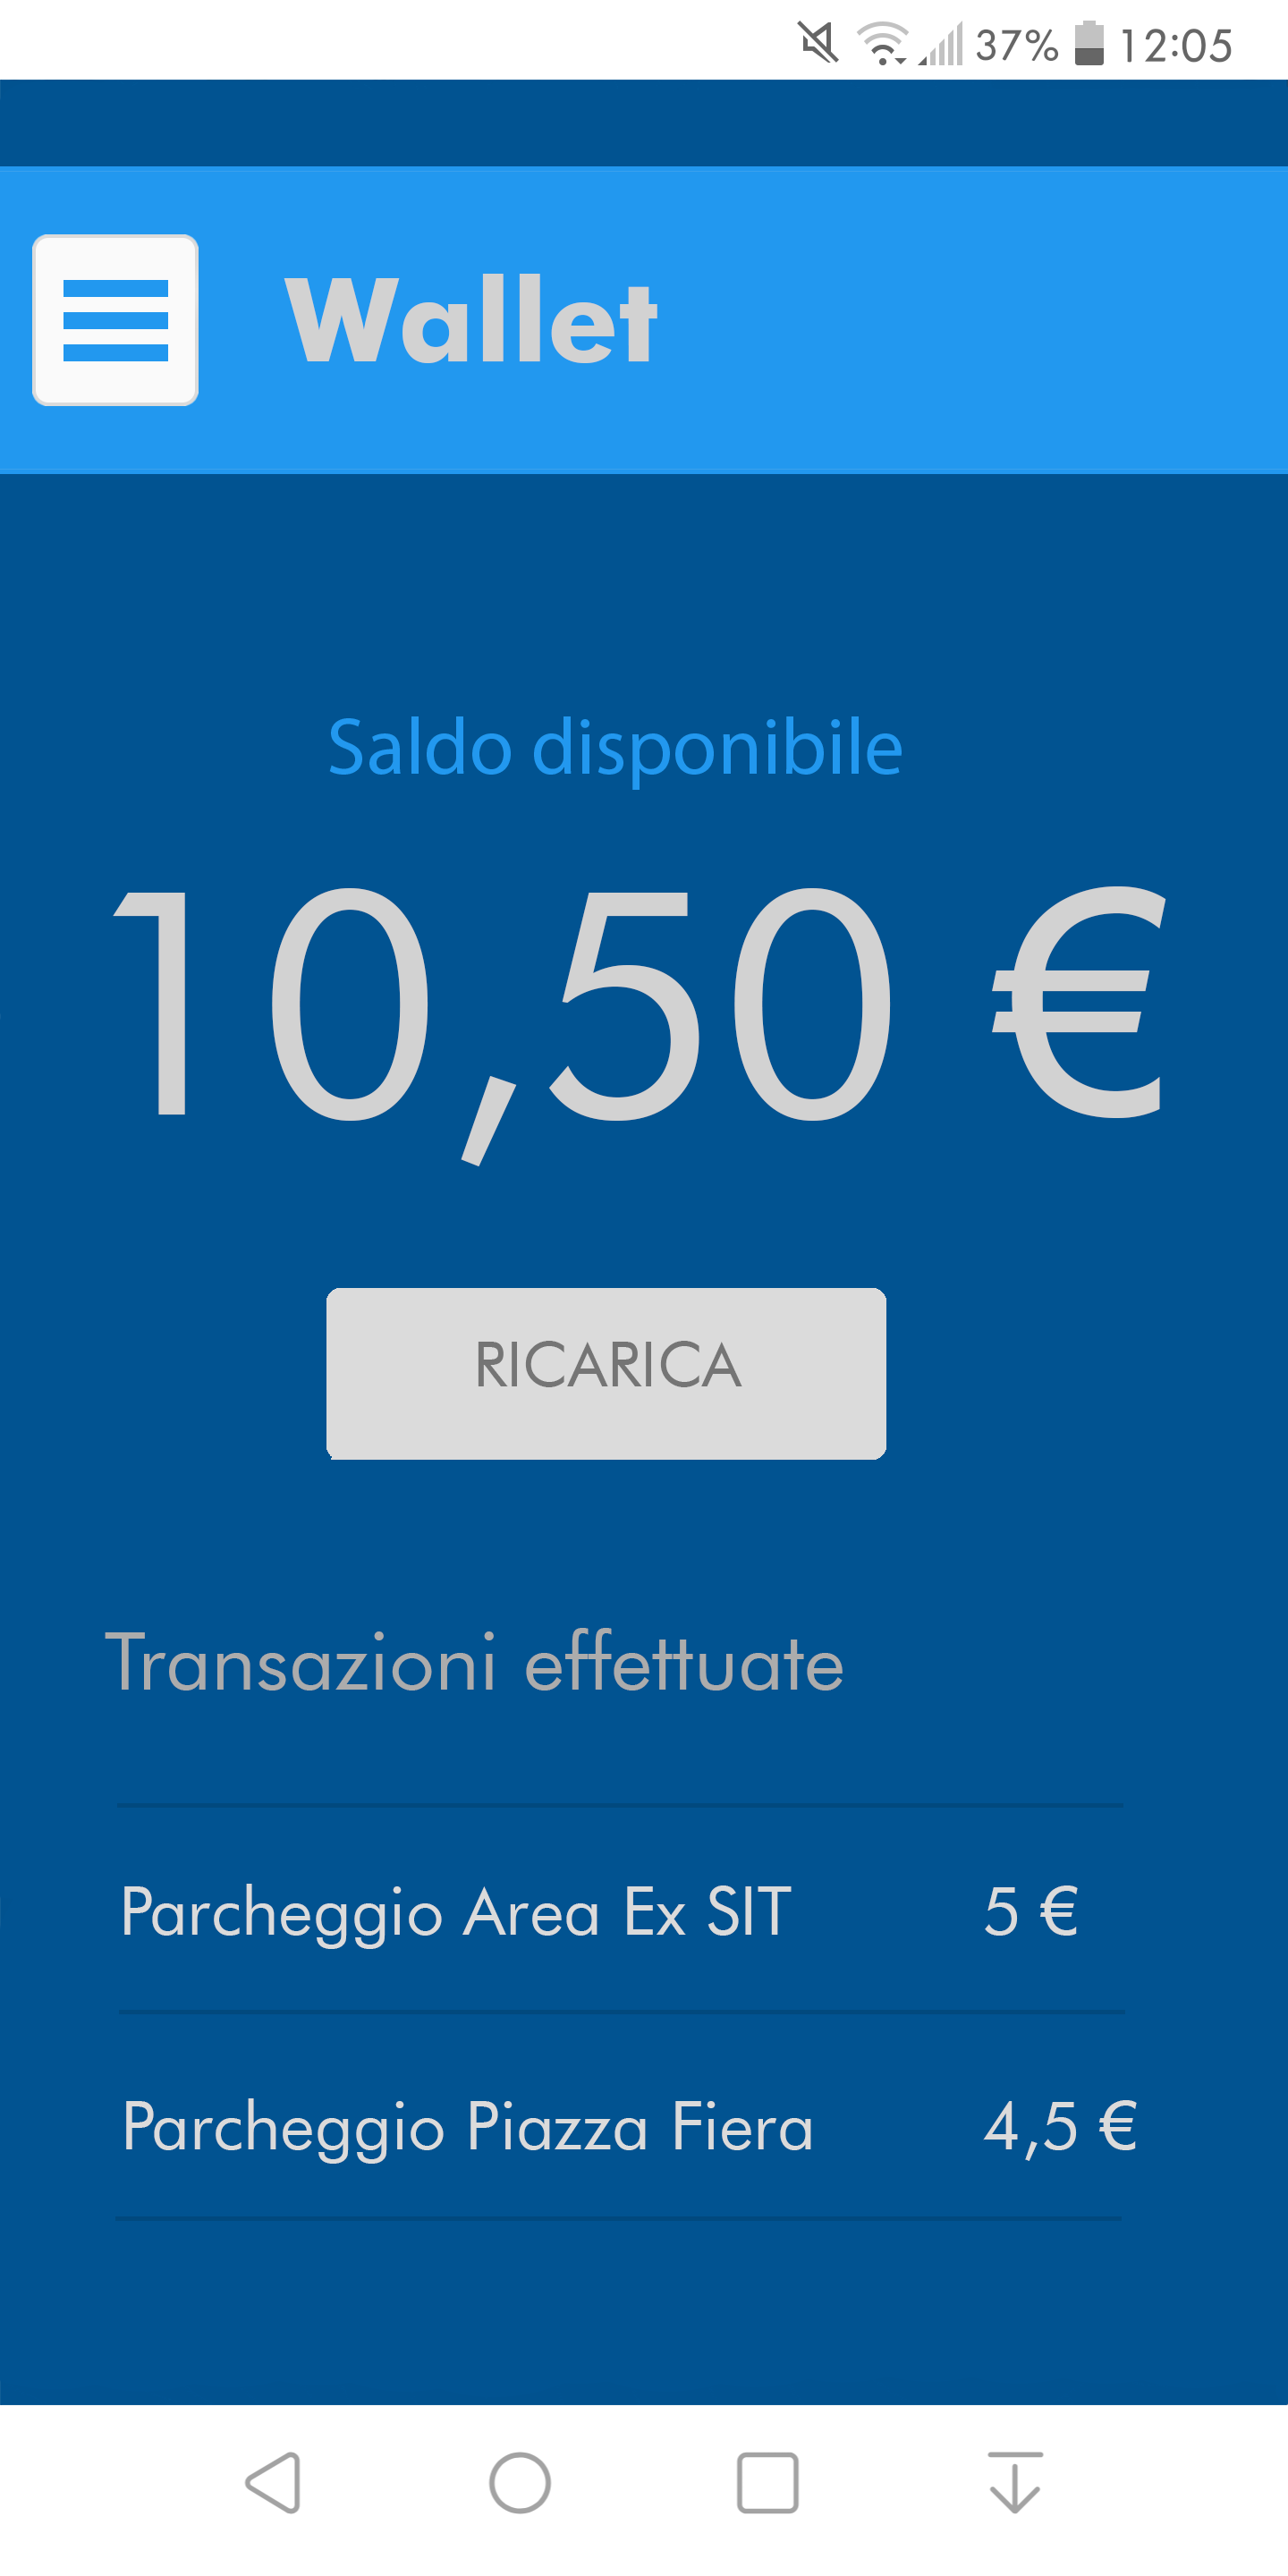
\includegraphics[scale=0.07,keepaspectratio, valign = c]{Img/wallet.png}}}
        \\
         & 
    \end{tabular}
    \label{tab:wallet}
\end{table}

\begin{table}[H]
    \centering
    \begin{tabular}{m{0.6\linewidth} c}
        Da questa sezione è possibile accedere alla lista delle prenotazioni effettuate. Il bottone con il cestino serve a cancellare una prenotazione, seguendo le indicazioni fornite in \ref{itm:RF21}.
        & 
        {\fbox{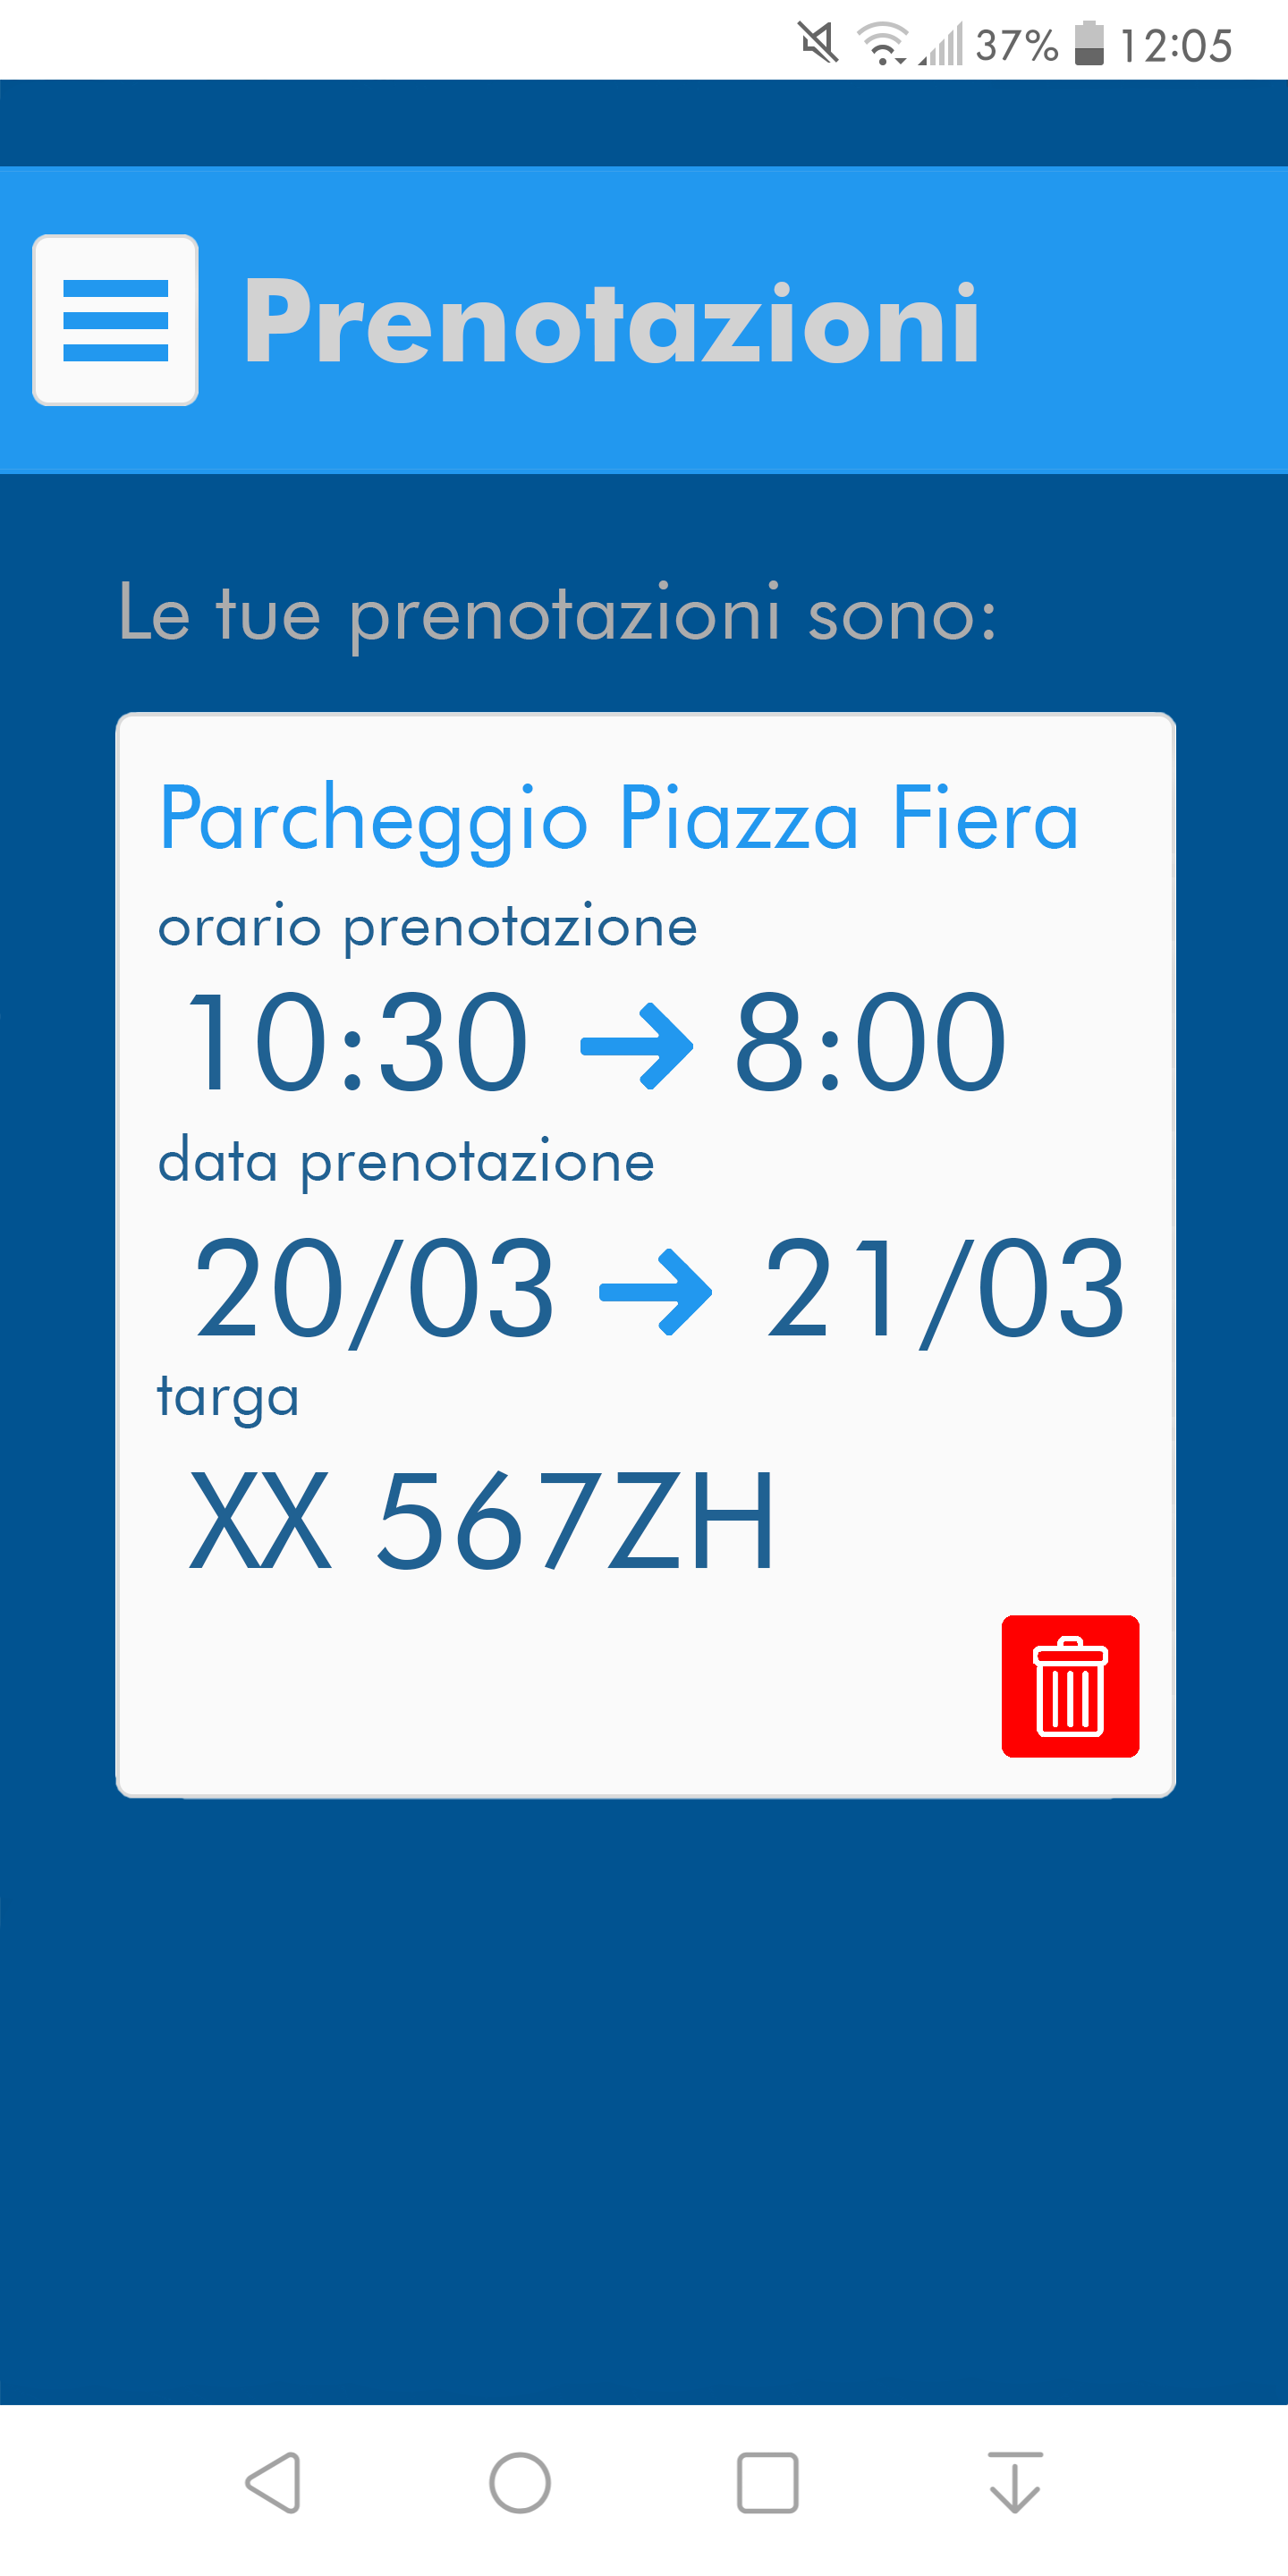
\includegraphics[scale=0.07,keepaspectratio, valign = c]{Img/listaPrenotazioni.png}}}
        \\
    \end{tabular}
    \label{tab:listaPrenotazioni}
\end{table}

\begin{table}[H]
    \centering
    \begin{tabular}{m{0.6\linewidth} c}
        Si può accedere in questa sezione selezionando "vedi profilo" dal menù ad hamburger. Qui l'utente può visualizzare i suoi dati e premendo il tasto "MODIFICA" può modificare la password come visto in RNF9.2, l'indirizzo email (la mail verrà verificata come alla prima registrazione vista nel punto) \ref{itm:RF2}.
        &  
        {\fbox{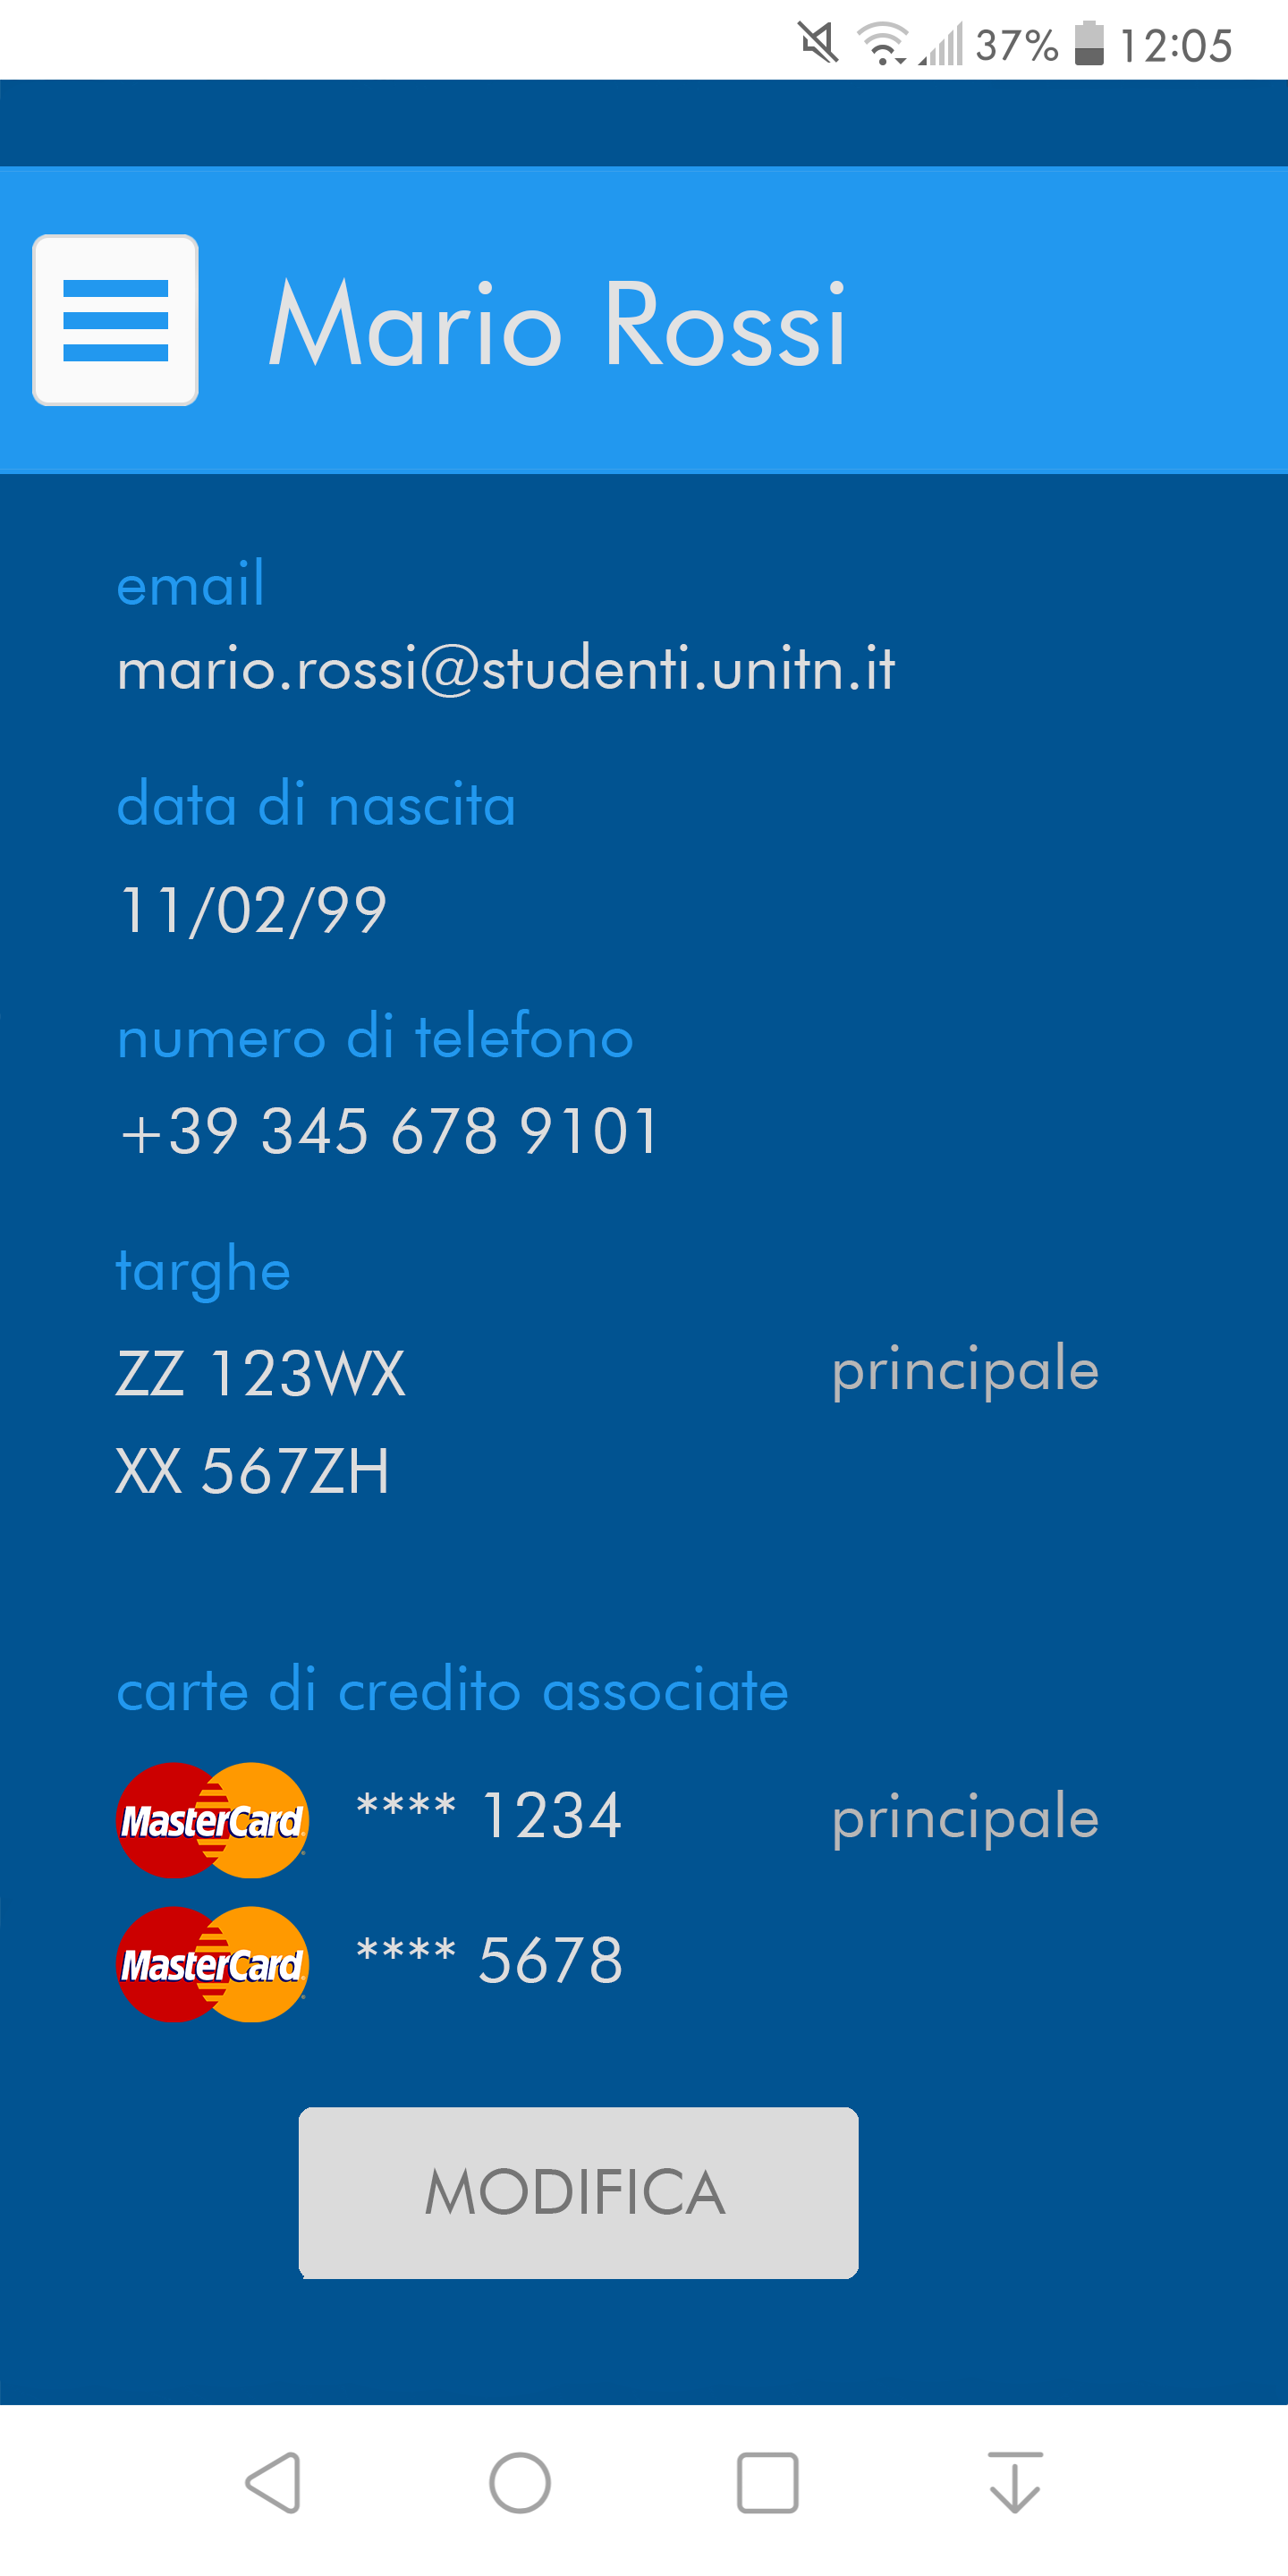
\includegraphics[scale=0.07,keepaspectratio, valign = c]{Img/datiPersonali.png}}}
        \\
    \end{tabular}
    \label{tab:my_label}
\end{table}

\begin{table}[H]
    \centering
    \begin{tabular}{m{0.6\linewidth} c}
        Questa sezione appare nel menù ad hamburger solo nel caso l'utente sia proprietario di un parcheggio. In questa sezione l'utente può modificare i dati del parcheggio e con il tasto "+" può aggiungere un parcheggio, nel caso ne possieda più di uno.
        & 
        {\fbox{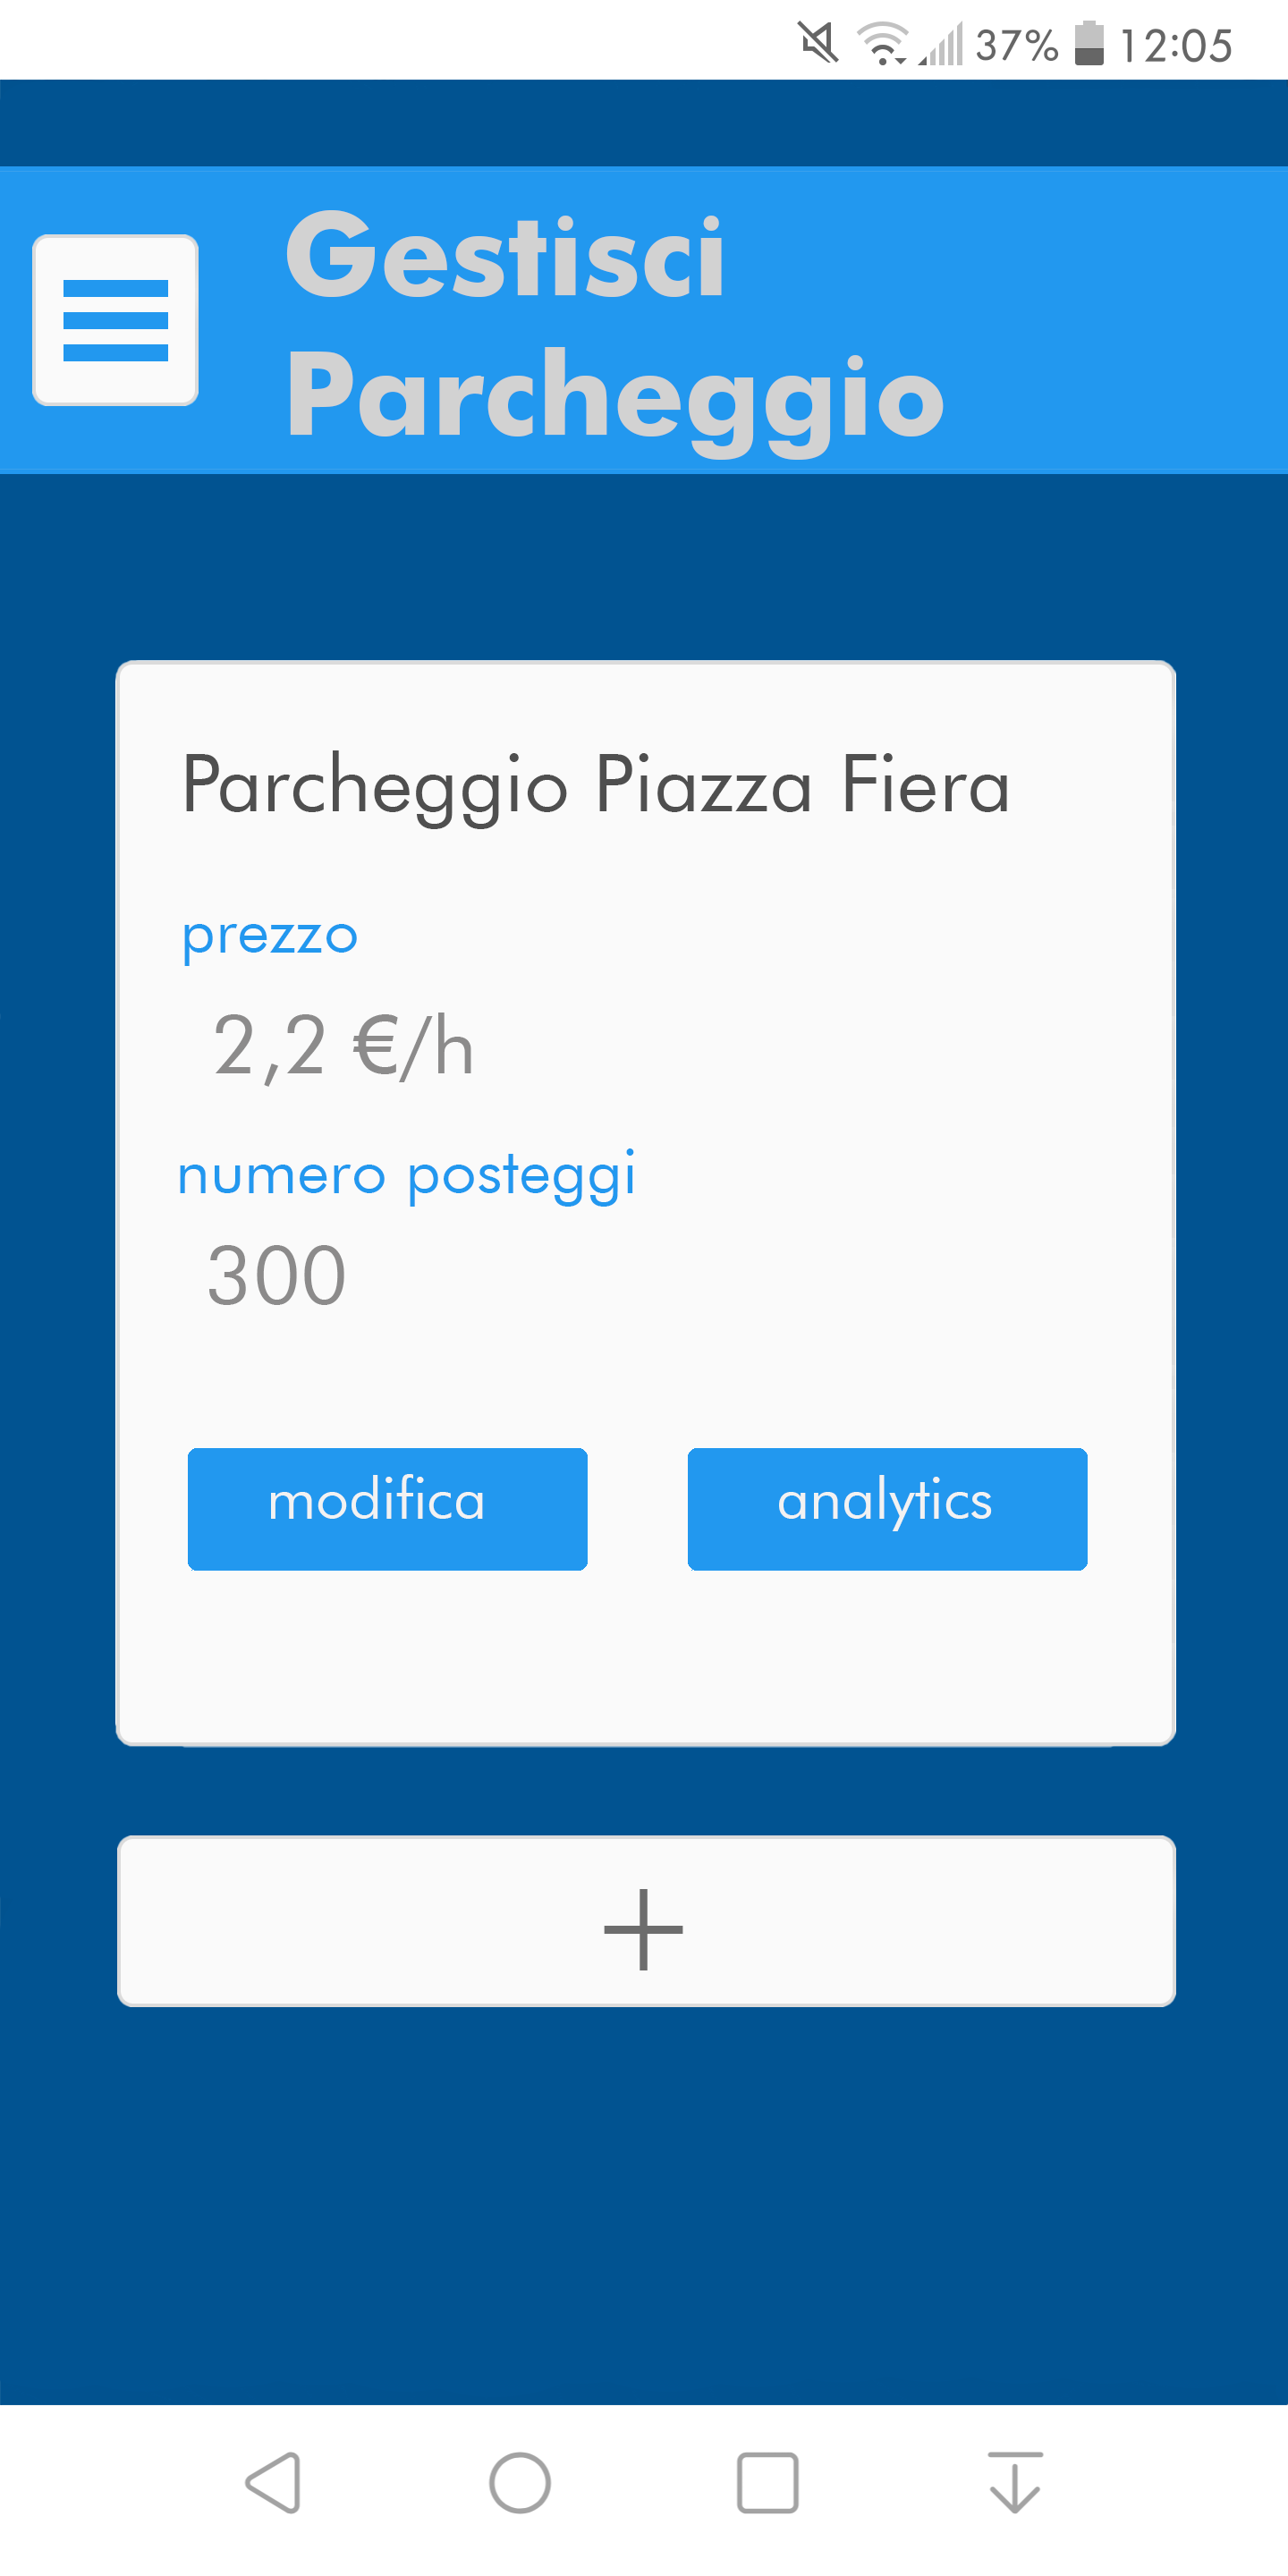
\includegraphics[scale=0.07,keepaspectratio, valign = c]{Img/gestisciParcheggio.png}}}
        \\
    \end{tabular}
    \label{tab:gestisciParcheggio}
\end{table}

\pagebreak
Alcune schermate del menù ad hamburger sono state omesse perché facilmente implementabili e con somiglianza ad altre rappresentate sopra:
\begin{itemize}
    \item "possiedi un parcheggio?" porta ad una finestra di registrazione simile all'immagine , inserendo nome del parcheggio, posti disponibili, città, via, CAP, tariffa oraria e orari di apertura del parcheggio. Alla fine della compilazione del form viene richiesto di caricare un file pdf/immagine che attesta la proprietà dell'immobile.
    \item "Contattaci" porta ad una schermata contenente una sezione in cui si descrive il problema o la domanda ed in basso un bottone con scritto "INVIA" che invia il form ad una mail di un centro assistenza.
    \item "Log Out" permette all'utente di effettuare il log out dall'applicazione. In questo caso al prossimo avvio verrà riportato alla schermata di accesso.
\end{itemize}